% Downloaded from http://www.dfcd.net/articles/latex/latex.html
% Modified by CC He.
% Notes on how to use this header is on Dropbox/Latex_Templates/LaTeX_for_Physicists/README.md
% ***********************************************************
% ******************* PHYSICS HEADER ************************
% ***********************************************************
% Version 2

\documentclass[12pt]{article}
\usepackage{setspace}
\usepackage{amsmath} % AMS Math Package
%\usepackage{fontspec,unicode-math}
%\usepackage{amsthm} % Theorem Formatting
\usepackage{amssymb}	% Math symbols such as \mathbb
\usepackage{units}
\usepackage{listings}
\usepackage{hyperref}
\usepackage{graphicx} % Allows for eps images
\usepackage{multicol} % Allows for multiple columns
\usepackage[dvips,letterpaper,margin=0.75in,bottom=0.5in]{geometry}
\usepackage{natbib}
\usepackage{float}

% Define ads acronyms
\newcommand{\apj}{ApJ}
\newcommand{\apjl}{ApJL}
\newcommand{\apjs}{ApJS}
\newcommand{\aap}{A\&A}
\newcommand{\araa}{ARA\&A}
\newcommand{\ssr}{SSR}
\newcommand{\mnras}{MNRAS}


 % Sets margins and page size
\pagestyle{empty} % Removes page numbers
%\pagestyle{fancy}
\makeatletter % Need for anything that contains an @ command 

\newcommand{\code}{\lstinline}
\renewcommand{\tt}{\texttt}
\newcommand{\m}{\textrm}
\renewcommand{\maketitle} % Redefine maketitle to conserve space
{ \begingroup \vskip 10pt \begin{center} \large {\bf \@title}
	\vskip 10pt \large \@author \hskip 20pt \@date \end{center}
  \vskip 10pt \endgroup \setcounter{footnote}{0} }
\makeatother % End of region containing @ commands
\renewcommand{\labelenumi}{(\alph{enumi})} % Use letters for enumerate
% \DeclareMathOperator{\Sample}{Sample}
\let\vaccent=\v % rename builtin command \v{} to \vaccent{}
\renewcommand{\v}[1]{\ensuremath{\mathbf{#1}}} % for vectors
\newcommand{\gv}[1]{\ensuremath{\mbox{\boldmath$ #1 $}}} 
% for vectors of Greek letters
\newcommand{\uv}[1]{\ensuremath{\mathbf{\hat{#1}}}} % for unit vector
\newcommand{\abs}[1]{\left| #1 \right|} % for absolute value
\newcommand{\avg}[1]{\left< #1 \right>} % for average
%\let\underdot=\d % rename builtin command \d{} to \underdot{}
\renewcommand{\d}[1]{\mathrm{d}#1} % for differential
\newcommand{\dd}[2]{\frac{\d{#1}}{\d{#2}}} % for derivatives
\newcommand{\ddd}[2]{\frac{\mathrm{d}^2 #1}{\d{#2^2}}} % for double 
%derivatives
\newcommand{\pd}[2]{\frac{\partial #1}{\partial #2}} 
% for partial derivatives
\newcommand{\pdd}[2]{\frac{\partial^2 #1}{\partial #2^2}} 
% for double partial derivatives
\newcommand{\pdc}[3]{\left( \frac{\partial #1}{\partial #2}
 \right)_{#3}} % for thermodynamic partial derivatives
\newcommand{\ket}[1]{\left| #1 \right>} % for Dirac bras
\newcommand{\bra}[1]{\left< #1 \right|} % for Dirac kets
\newcommand{\braket}[2]{\left< #1 \vphantom{#2} \right|
 \left. #2 \vphantom{#1} \right>} % for Dirac brackets
\newcommand{\matrixel}[3]{\left< #1 \vphantom{#2#3} \right|
 #2 \left| #3 \vphantom{#1#2} \right>} % for Dirac matrix elements
\newcommand{\grad}[1]{\gv{\nabla} #1} % for gradient
\let\divsymb=\div % rename builtin command \div to \divsymb
\renewcommand{\div}[1]{\gv{\nabla} \cdot #1} % for divergence
\newcommand{\curl}[1]{\gv{\nabla} \times #1} % for curl
\let\baraccent=\= % rename builtin command \= to \baraccent
\renewcommand{\=}[1]{\stackrel{#1}{=}} % for putting numbers above =
\newtheorem{prop}{Proposition}
\newtheorem{thm}{Theorem}[section]
\newtheorem{lem}[thm]{Lemma}
%\theoremstyle{definition}
\newtheorem{dfn}{Definition}
%\theoremstyle{remark}
%\newtheorem*{rmk}{Remark}


% Define \stretchint, a macro to input large integrals.
\usepackage{scalerel}[2016-12-29]
\def\stretchint#1{\vcenter{\hbox{\stretchto[440]{\displaystyle\int}{#1}}}}
\def\scaleint#1{\vcenter{\hbox{\scaleto[3ex]{\displaystyle\int}{#1}}}}
\def\bs{\mkern-12mu}


\begin{document}

\title{ASTR615 HW\#4}
\author{Group 4: ChongChong He \& Mohammed Khalil\\}
\date{\today}
\maketitle


\section{Problem 1}

\subsubsection*{2nd order leapfrog vs. 4th order Runge-Kutta for e = 0.5}

\begin{figure}[H]
	\centering
	\begin{minipage}[b]{0.48\linewidth}
		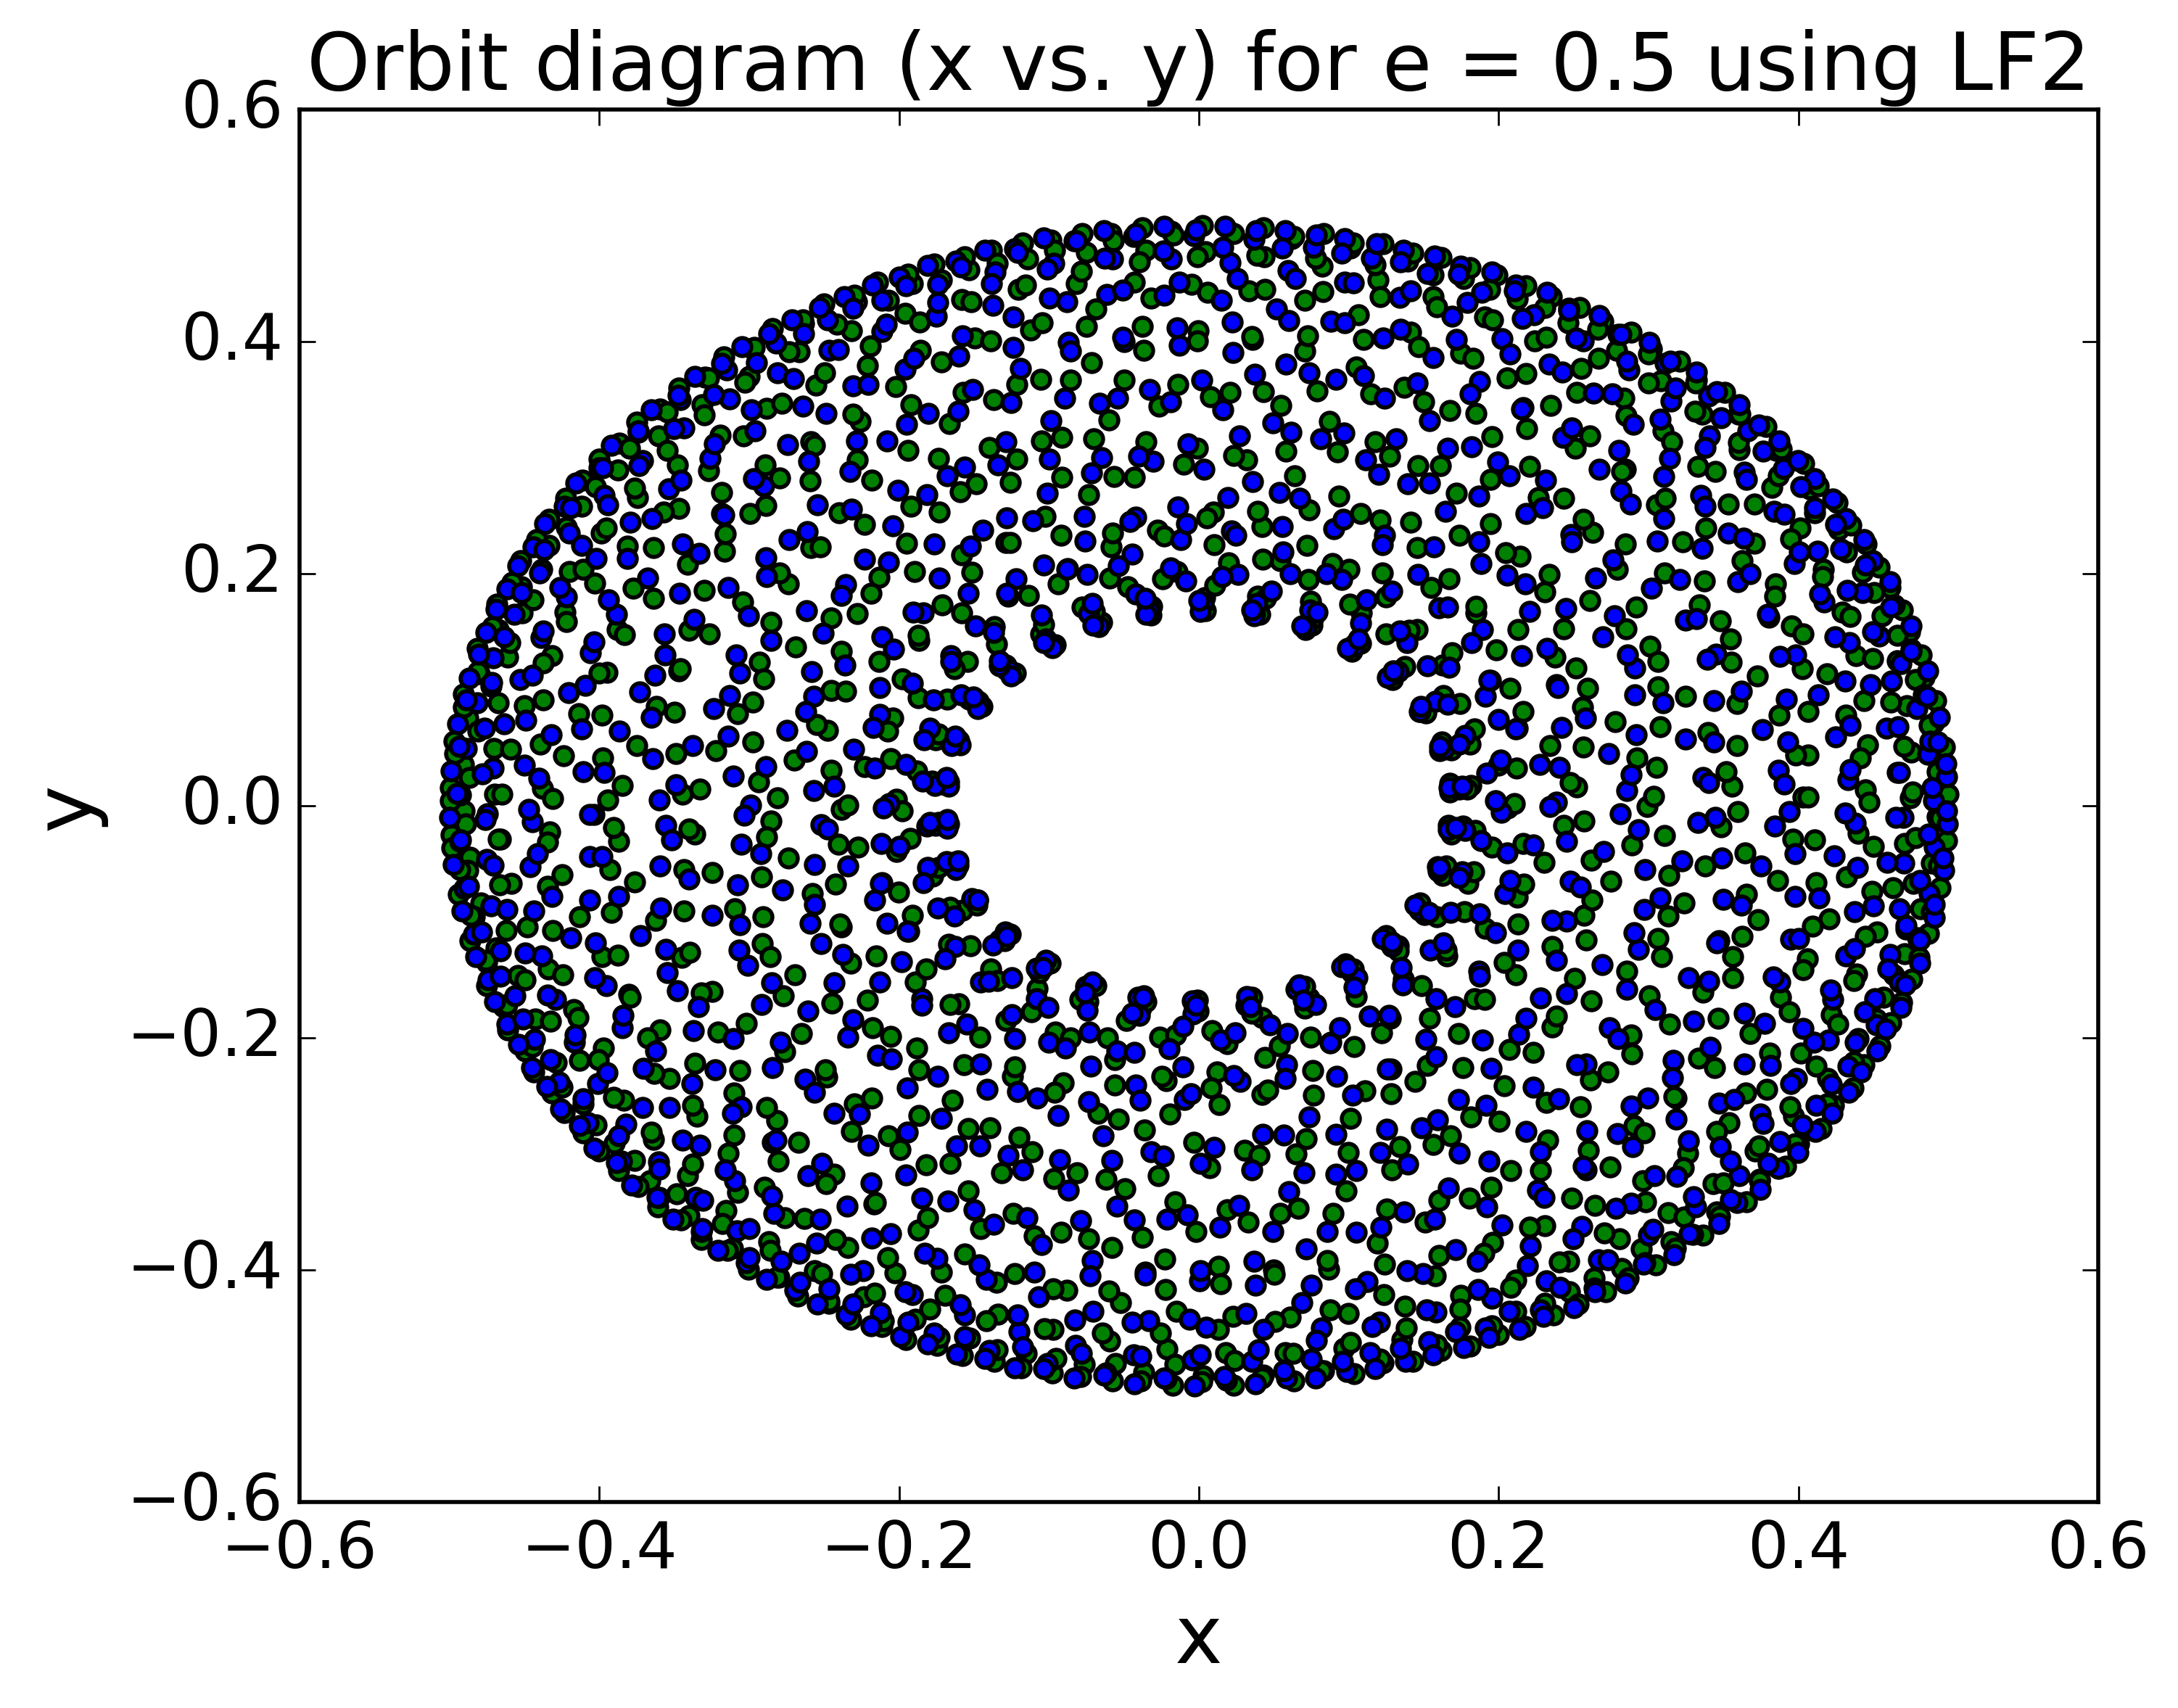
\includegraphics[width=\linewidth]{plots_p1/LF2_e05_xy.png}
		%\caption{\label{fig:lightstd}.}
	\end{minipage}
	%\quad
	\begin{minipage}[b]{0.48\linewidth}
		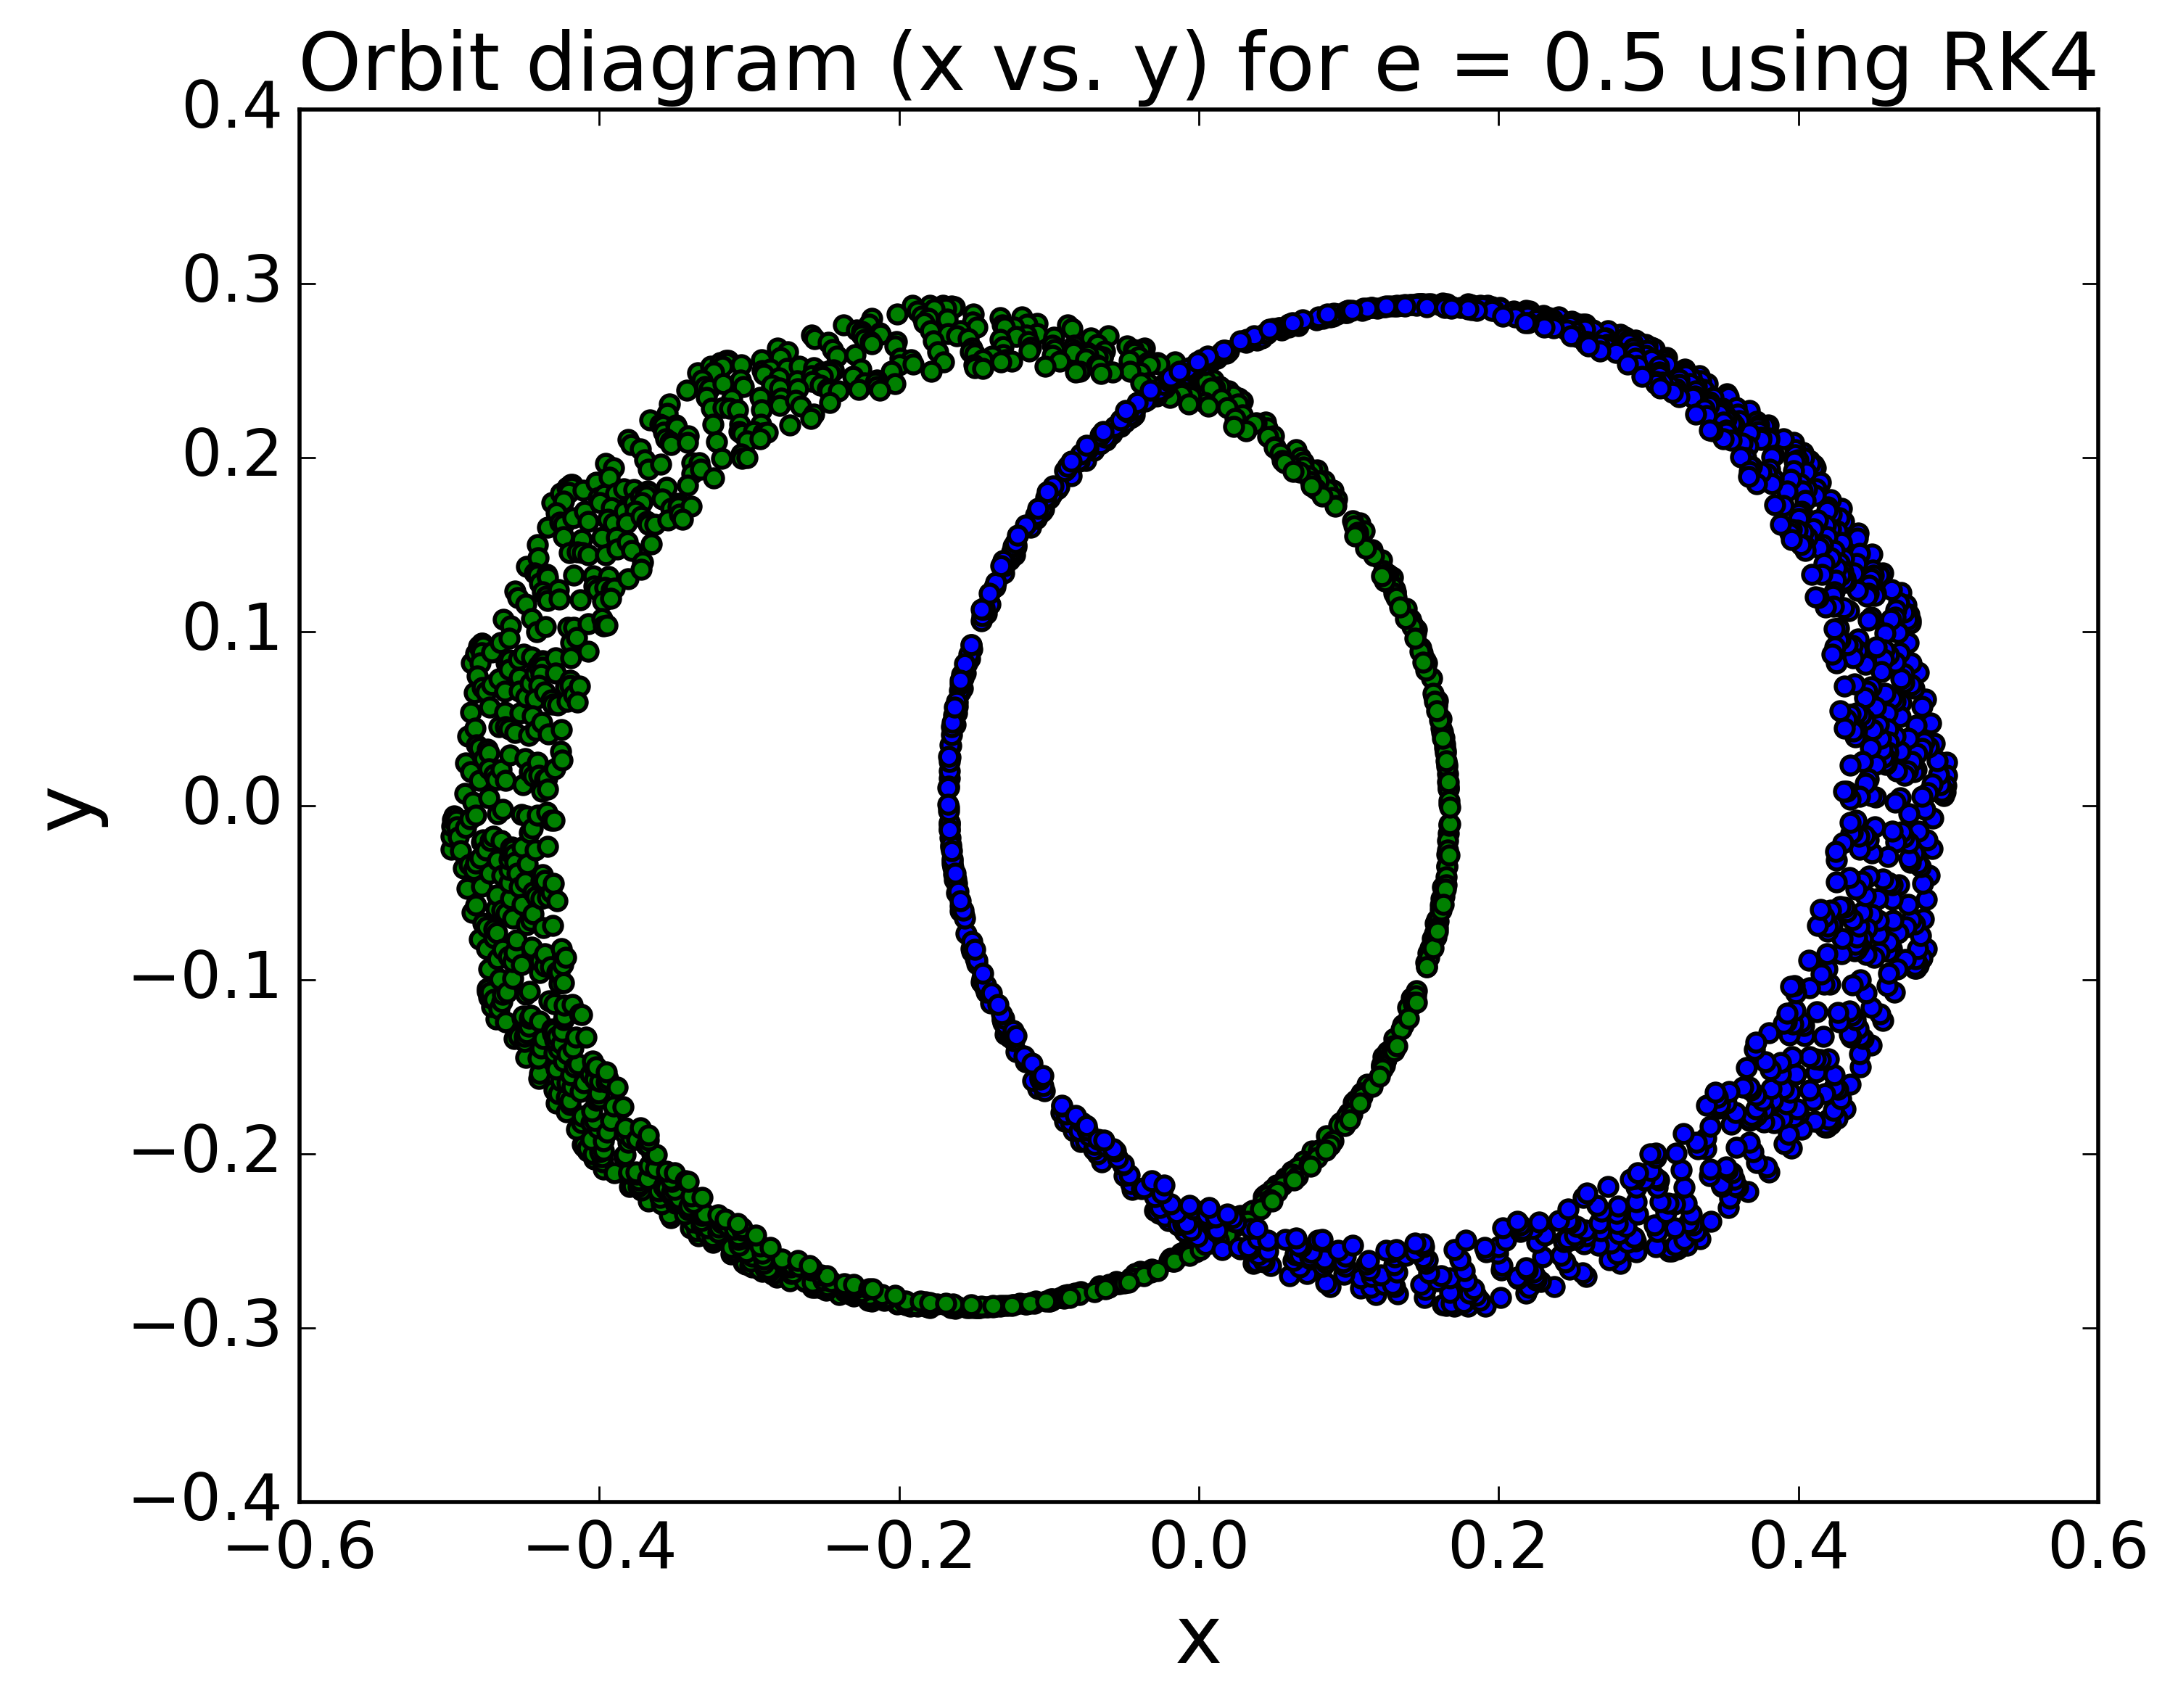
\includegraphics[width=\linewidth]{plots_p1/RK4_e05_xy.png}
	\end{minipage}
\end{figure}

\begin{figure}[H]
	\centering
	\begin{minipage}[b]{0.48\linewidth}
		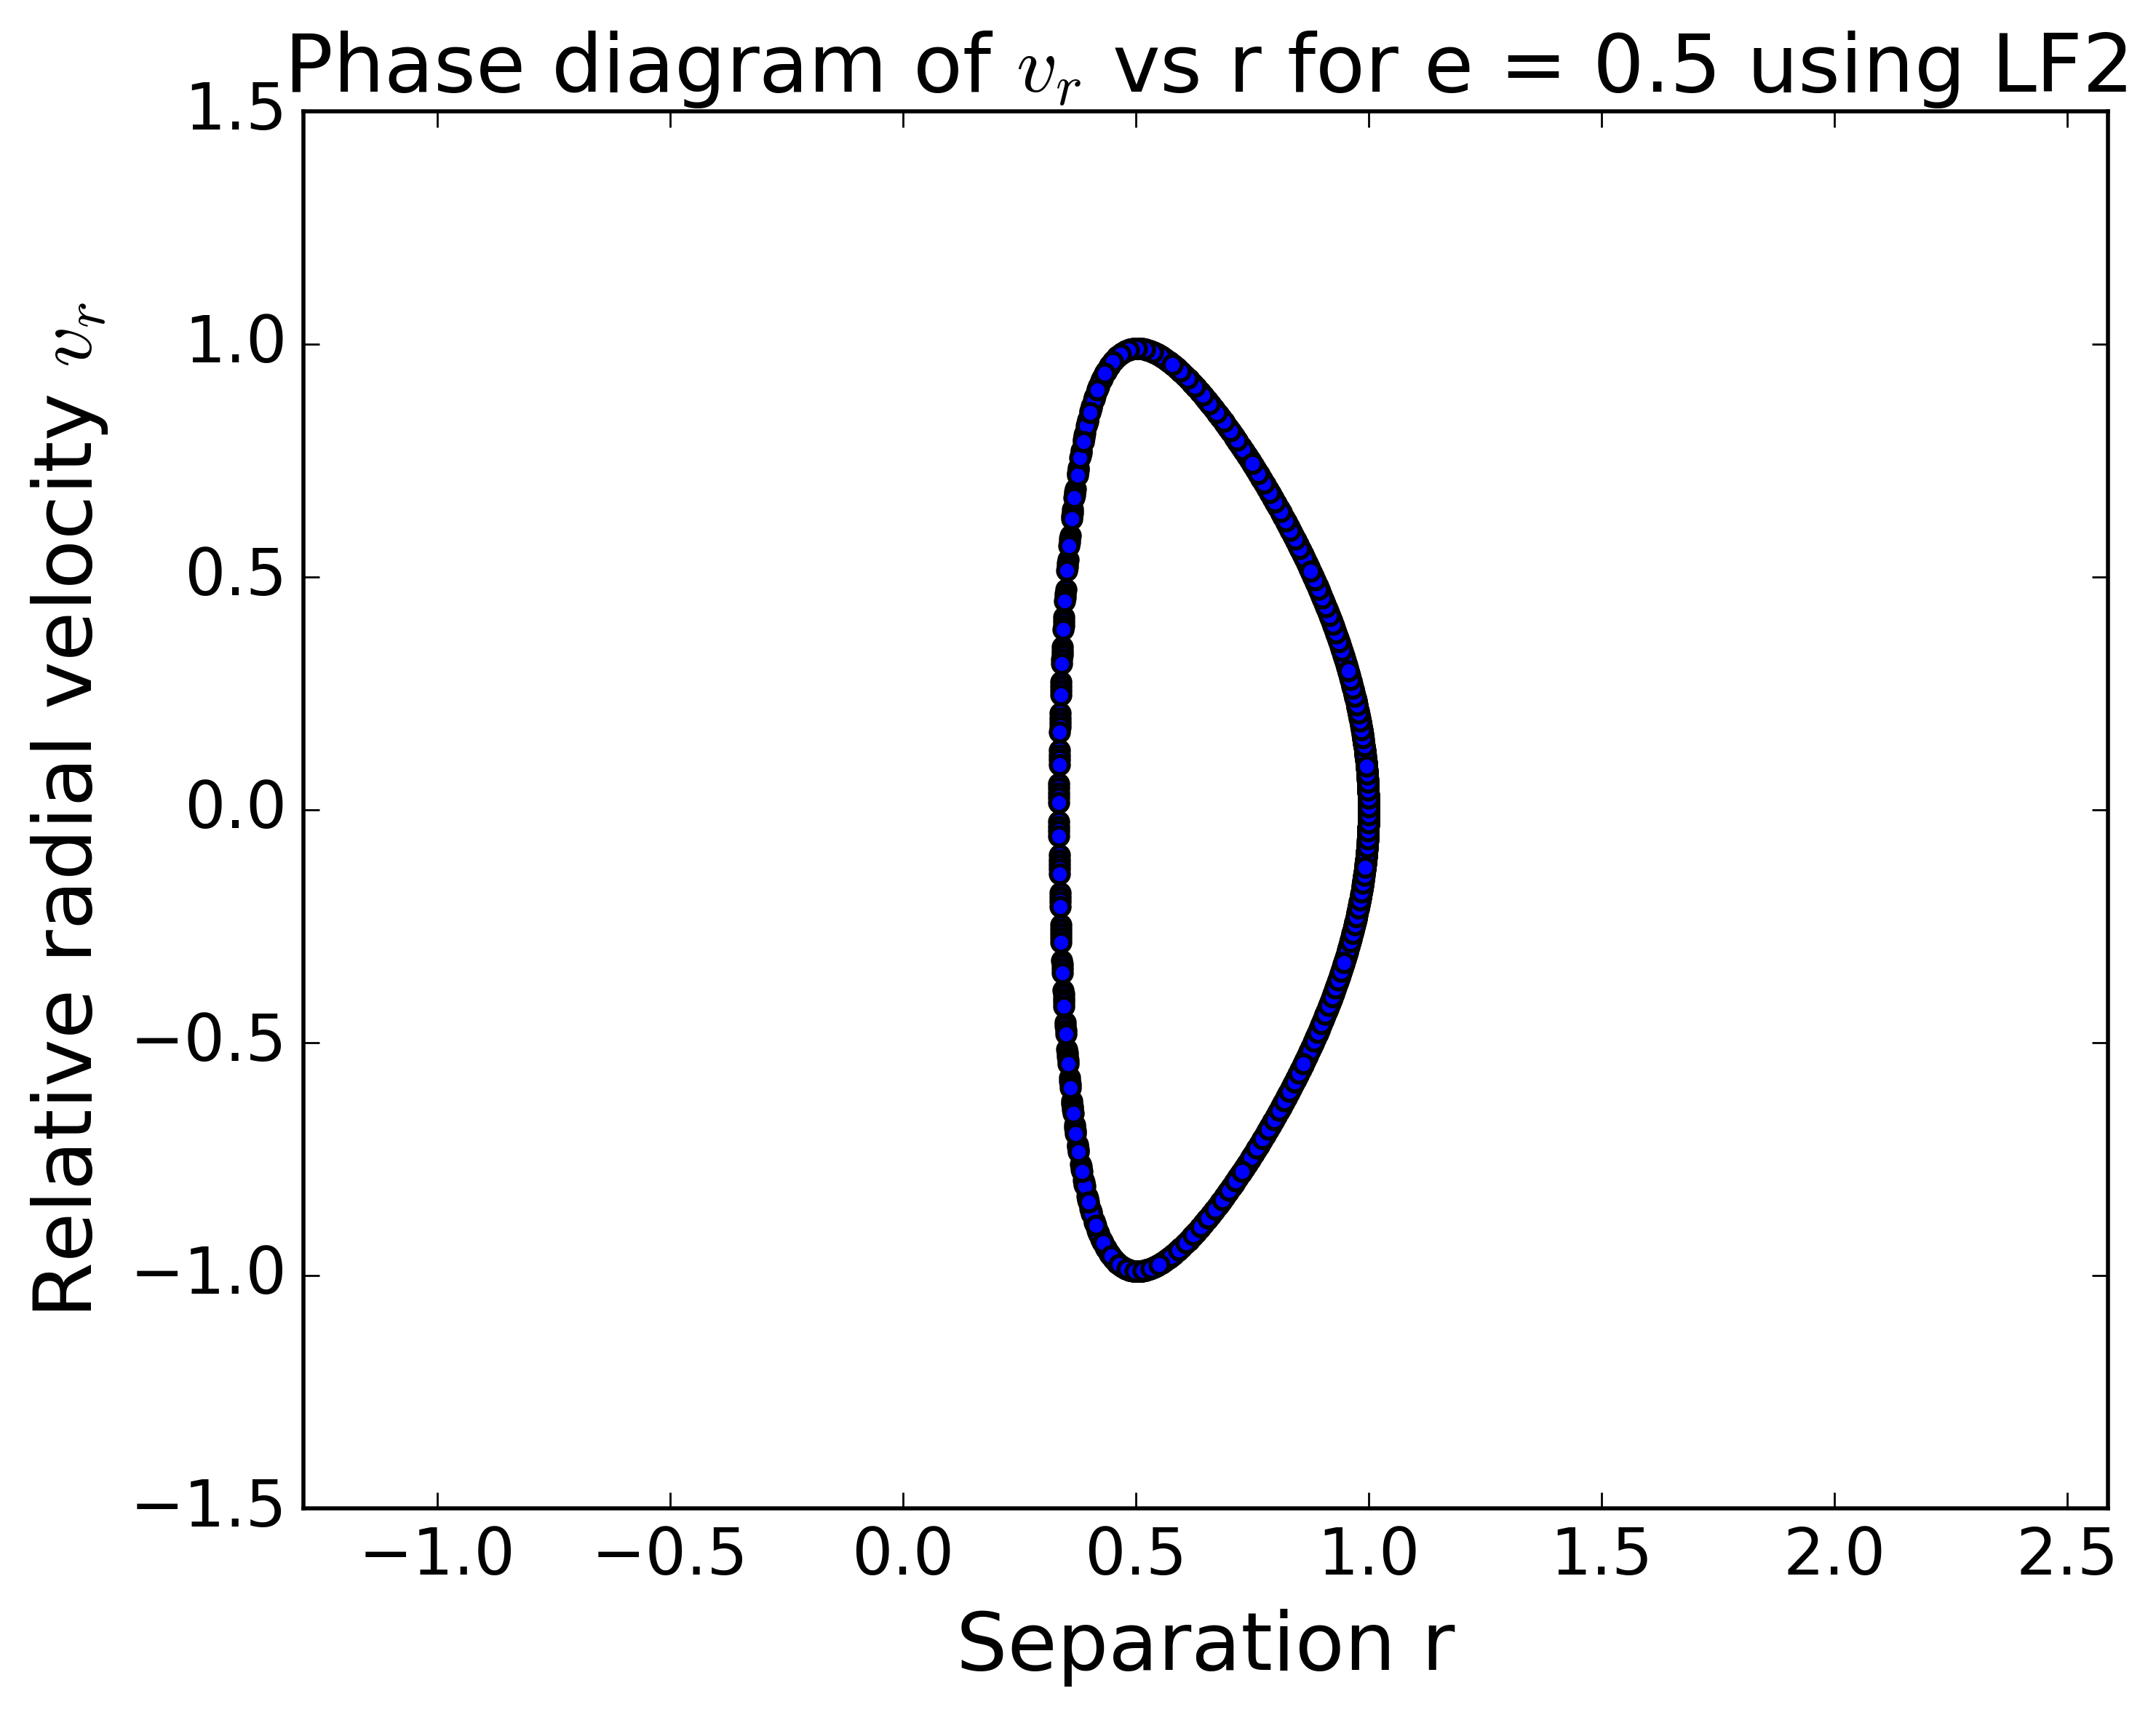
\includegraphics[width=\linewidth]{plots_p1/LF2_e05_rv.png}
		%\caption{\label{fig:lightstd}.}
	\end{minipage}
	%\quad
	\begin{minipage}[b]{0.48\linewidth}
		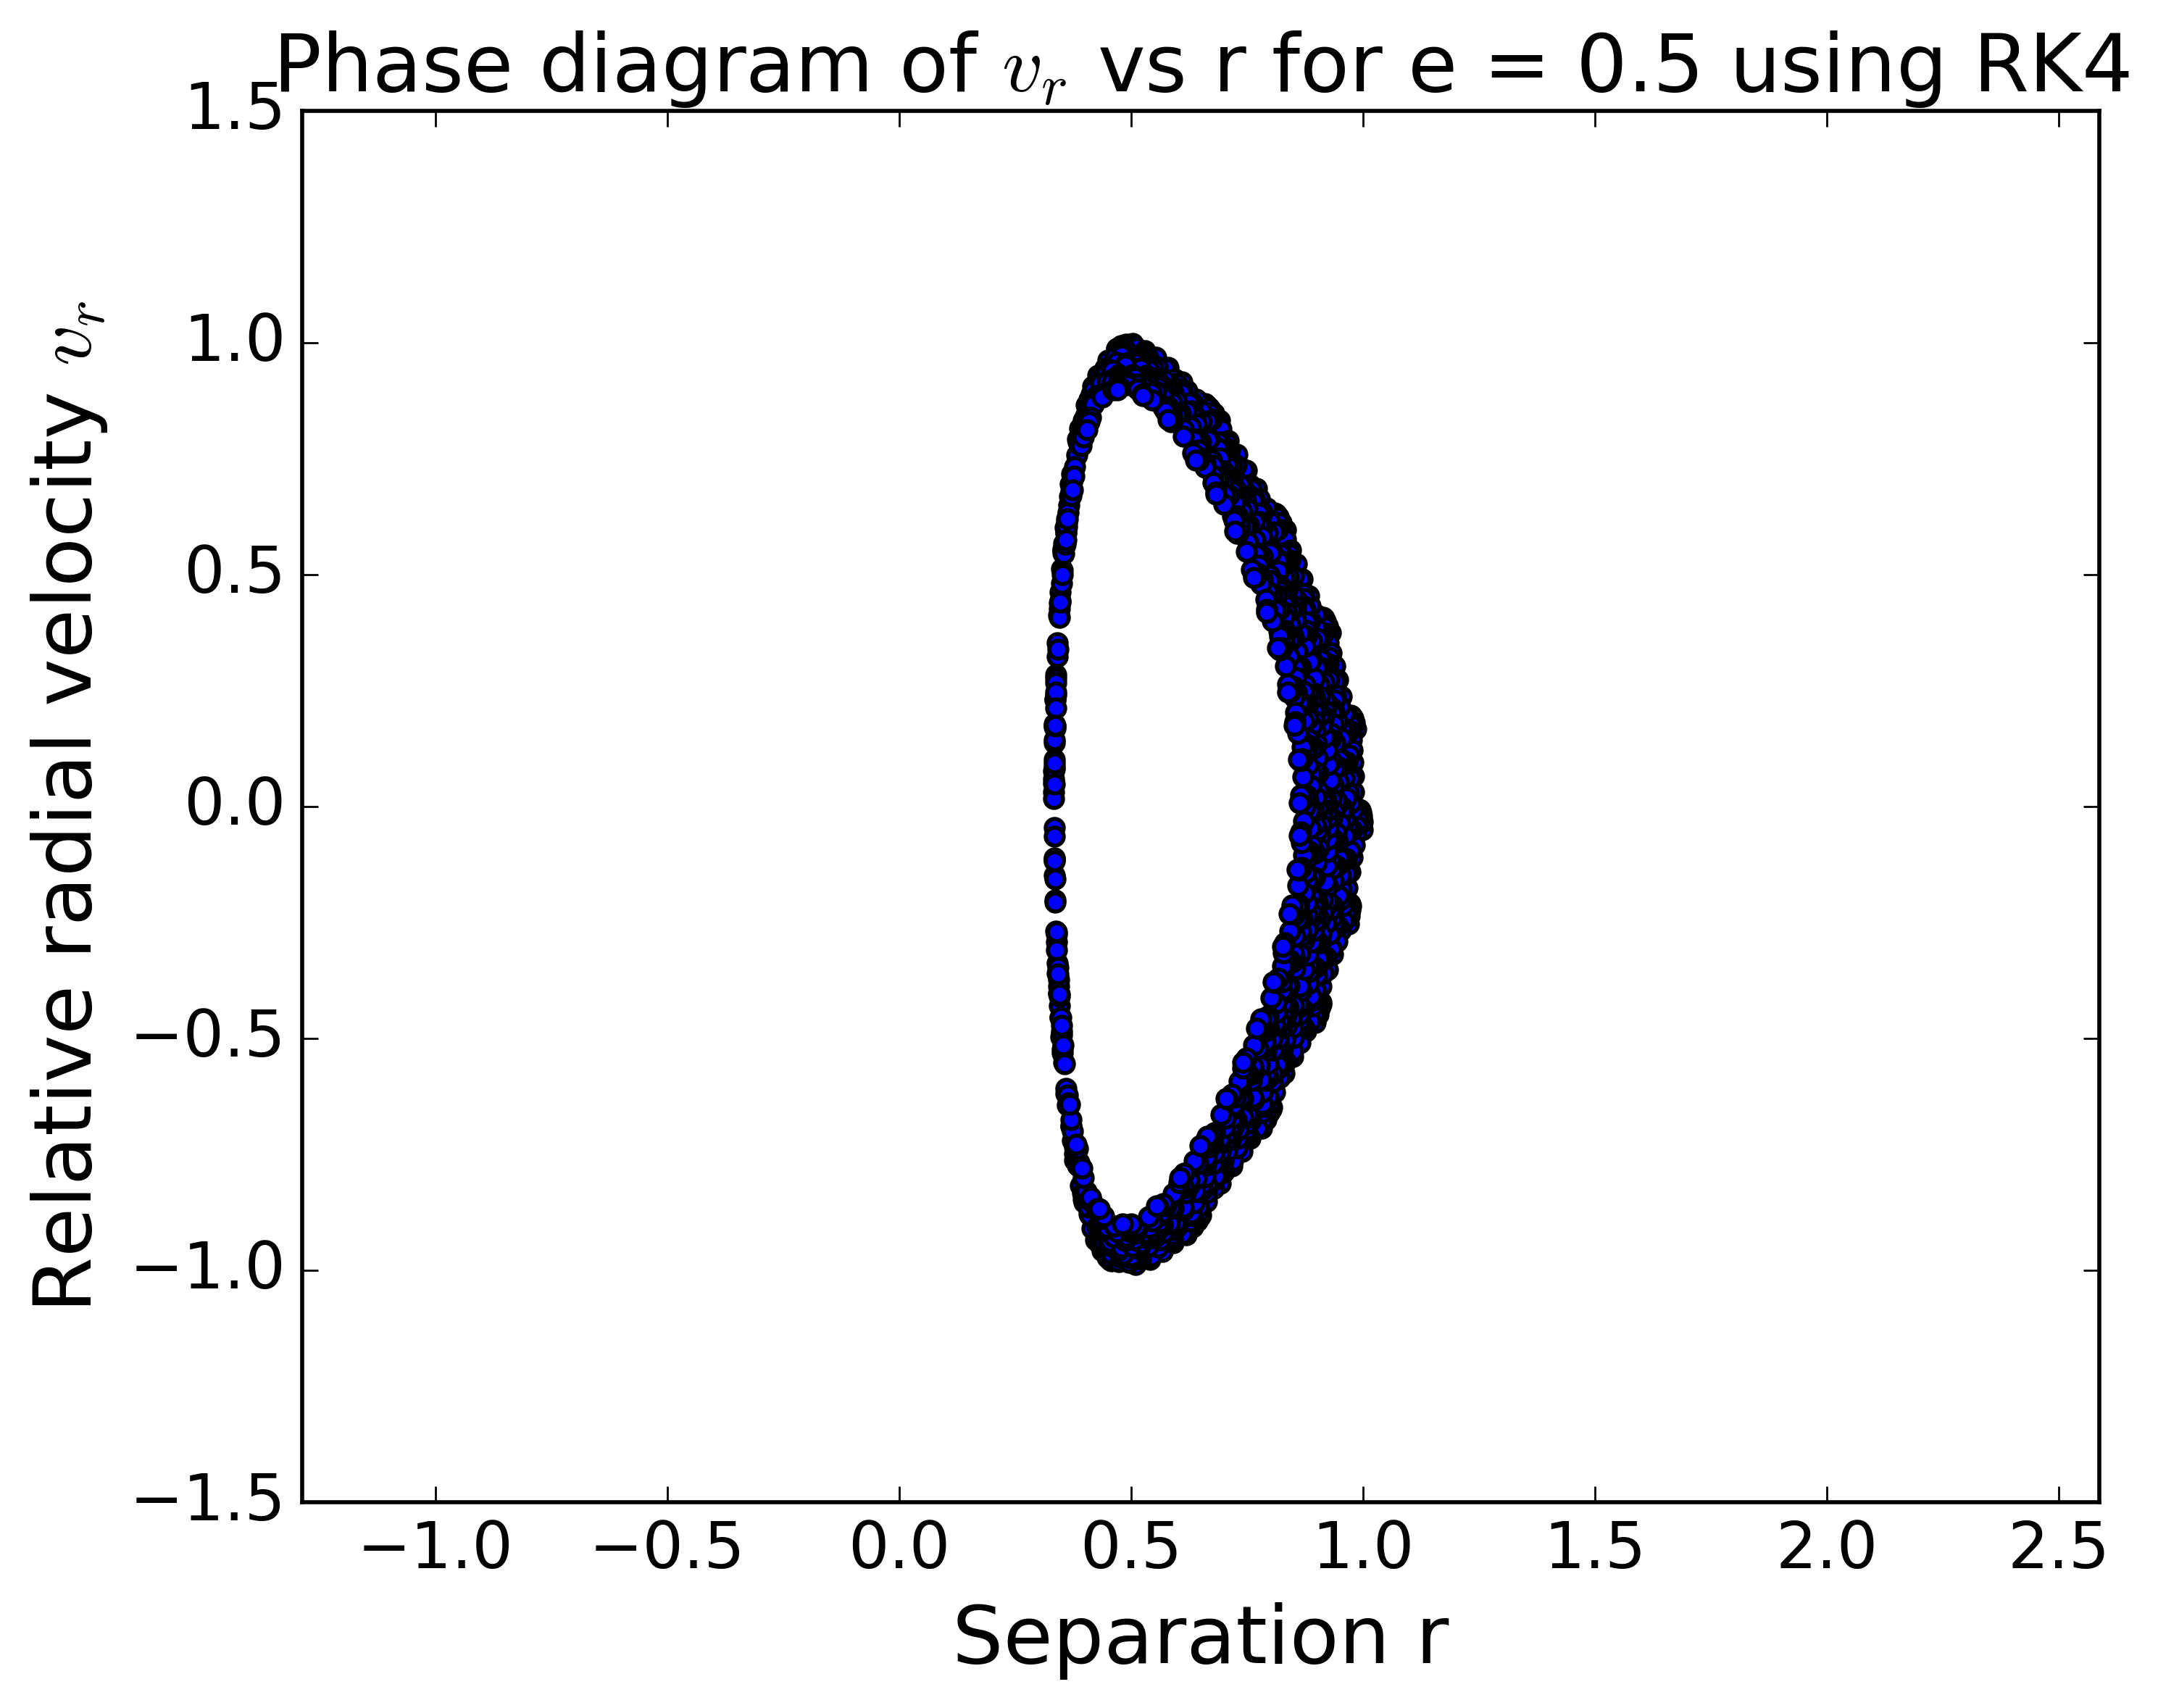
\includegraphics[width=\linewidth]{plots_p1/RK4_e05_rv.png}
	\end{minipage}
\end{figure}

\begin{figure}[H]
	\centering
	\begin{minipage}[b]{0.48\linewidth}
		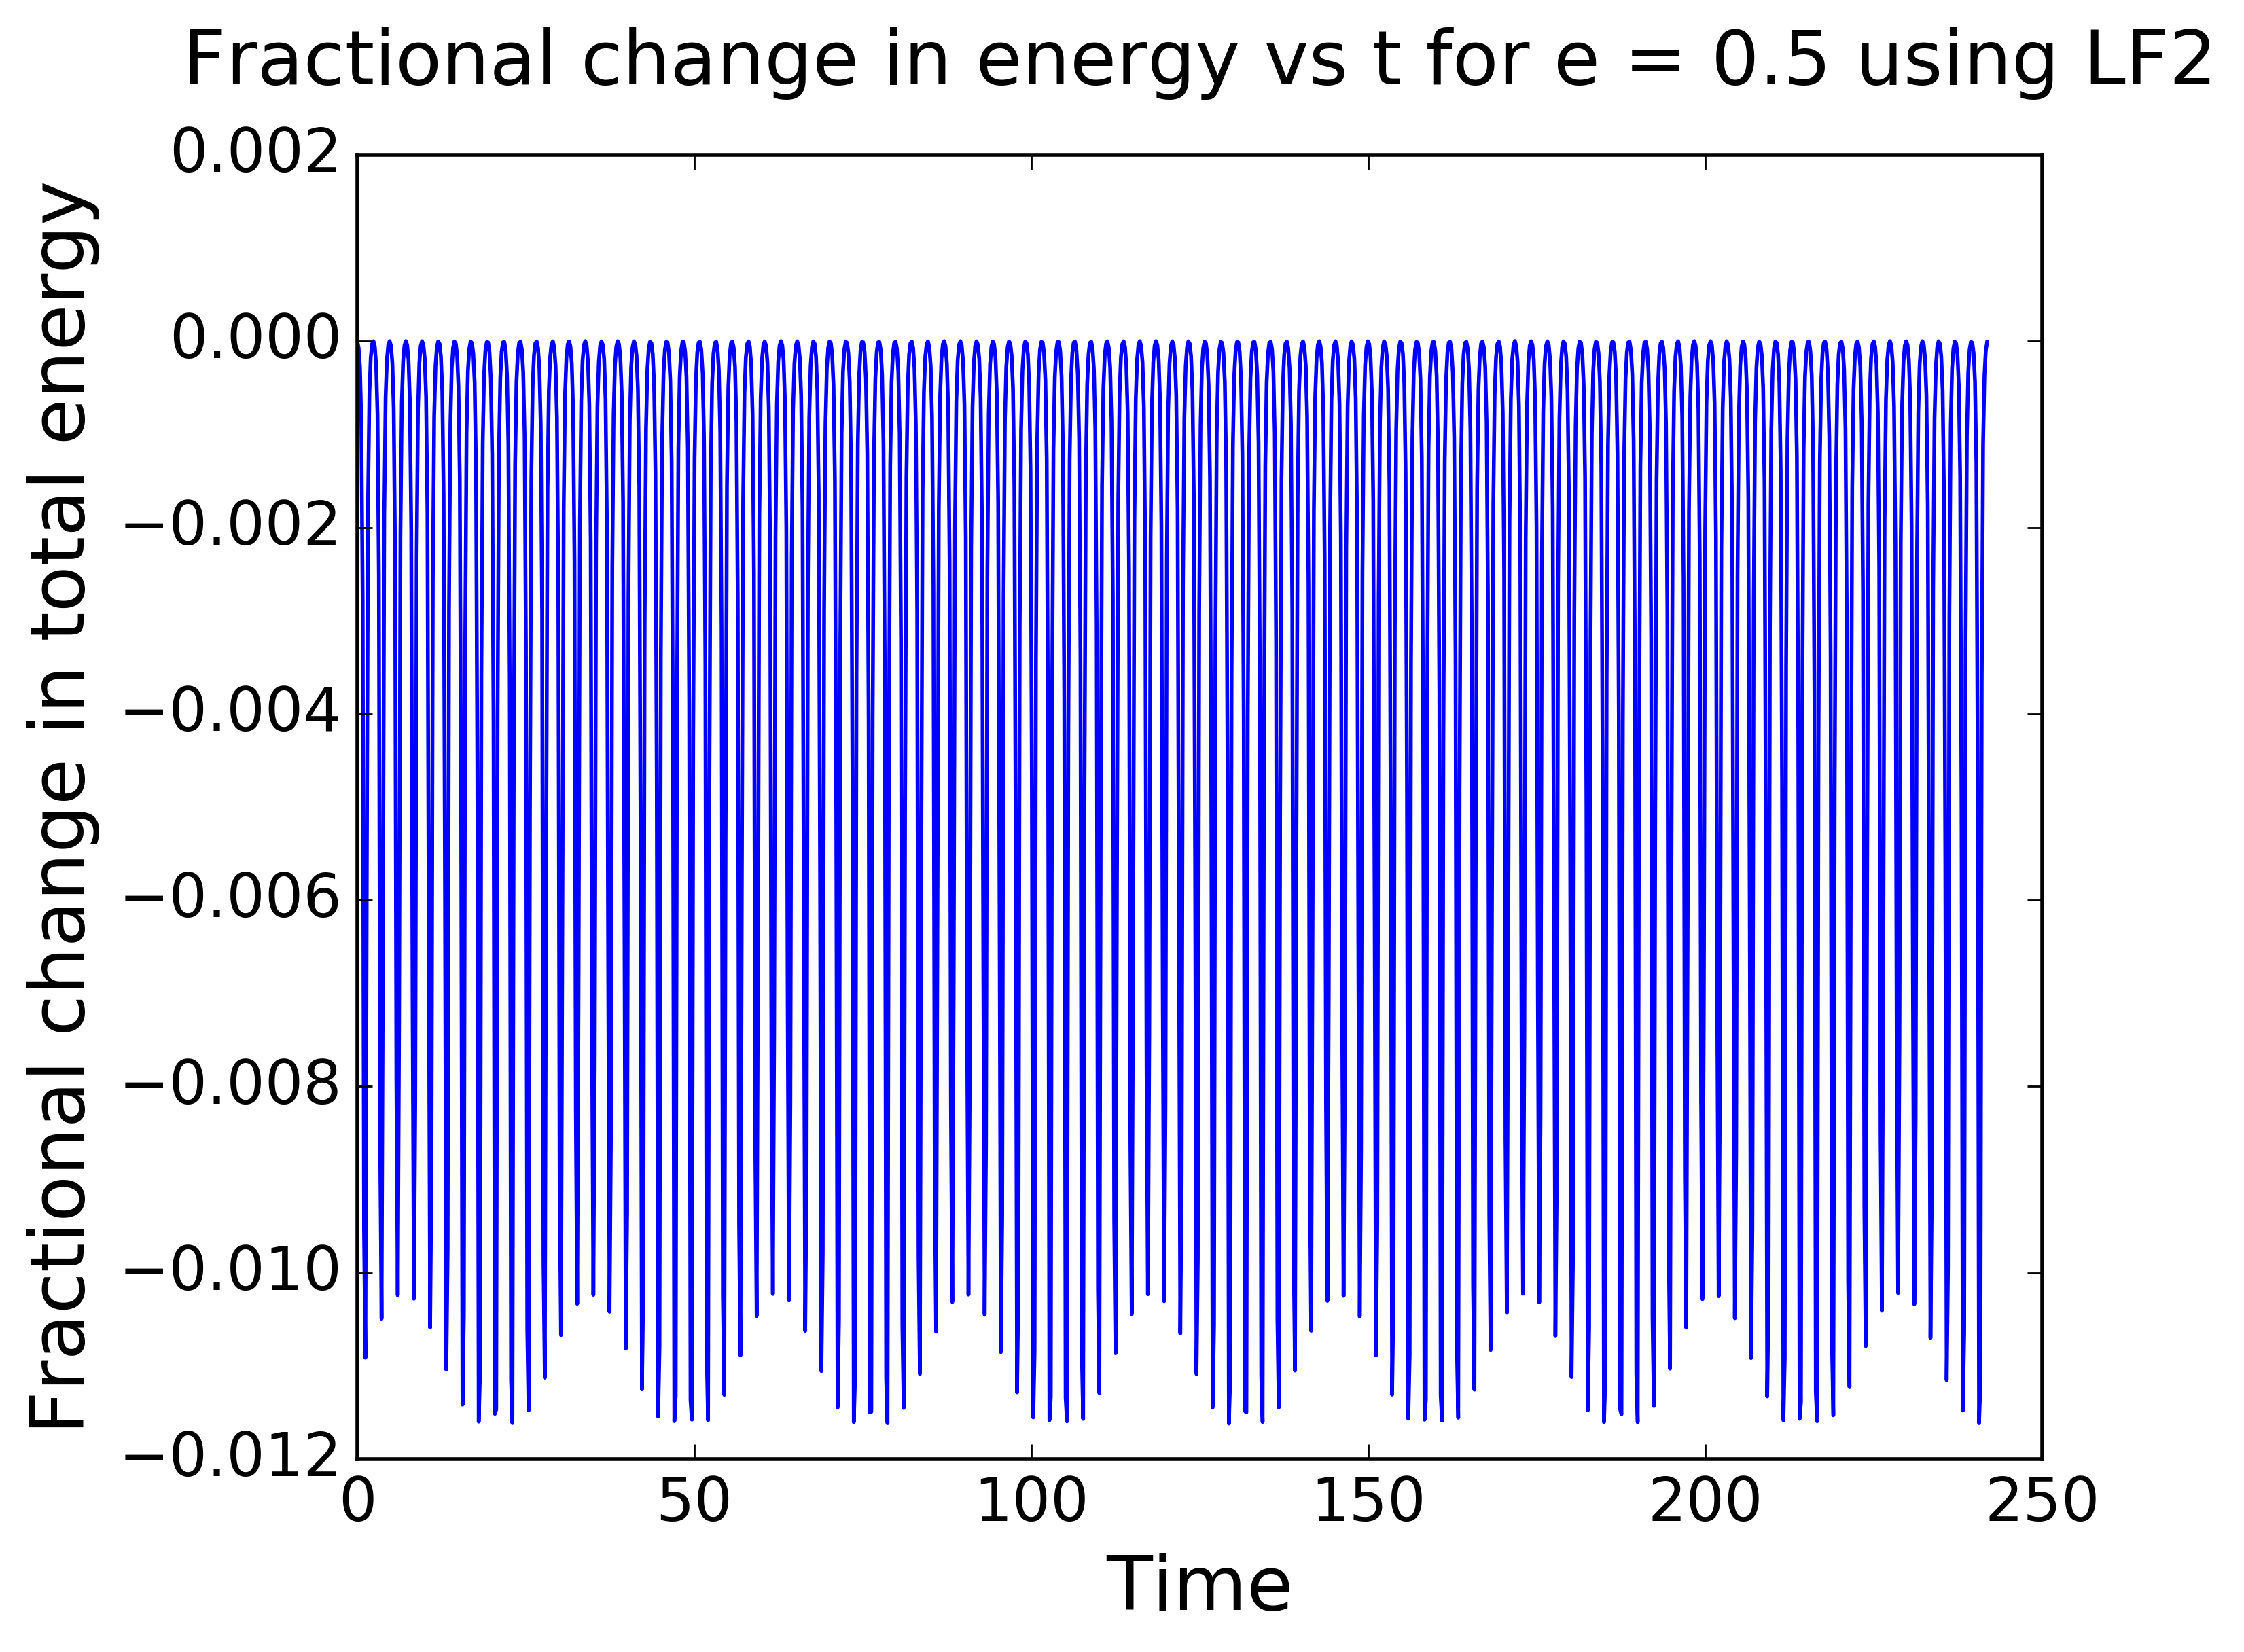
\includegraphics[width=\linewidth]{plots_p1/LF2_e05_energy.png}
		%\caption{\label{fig:lightstd}.}
	\end{minipage}
	%\quad
	\begin{minipage}[b]{0.48\linewidth}
		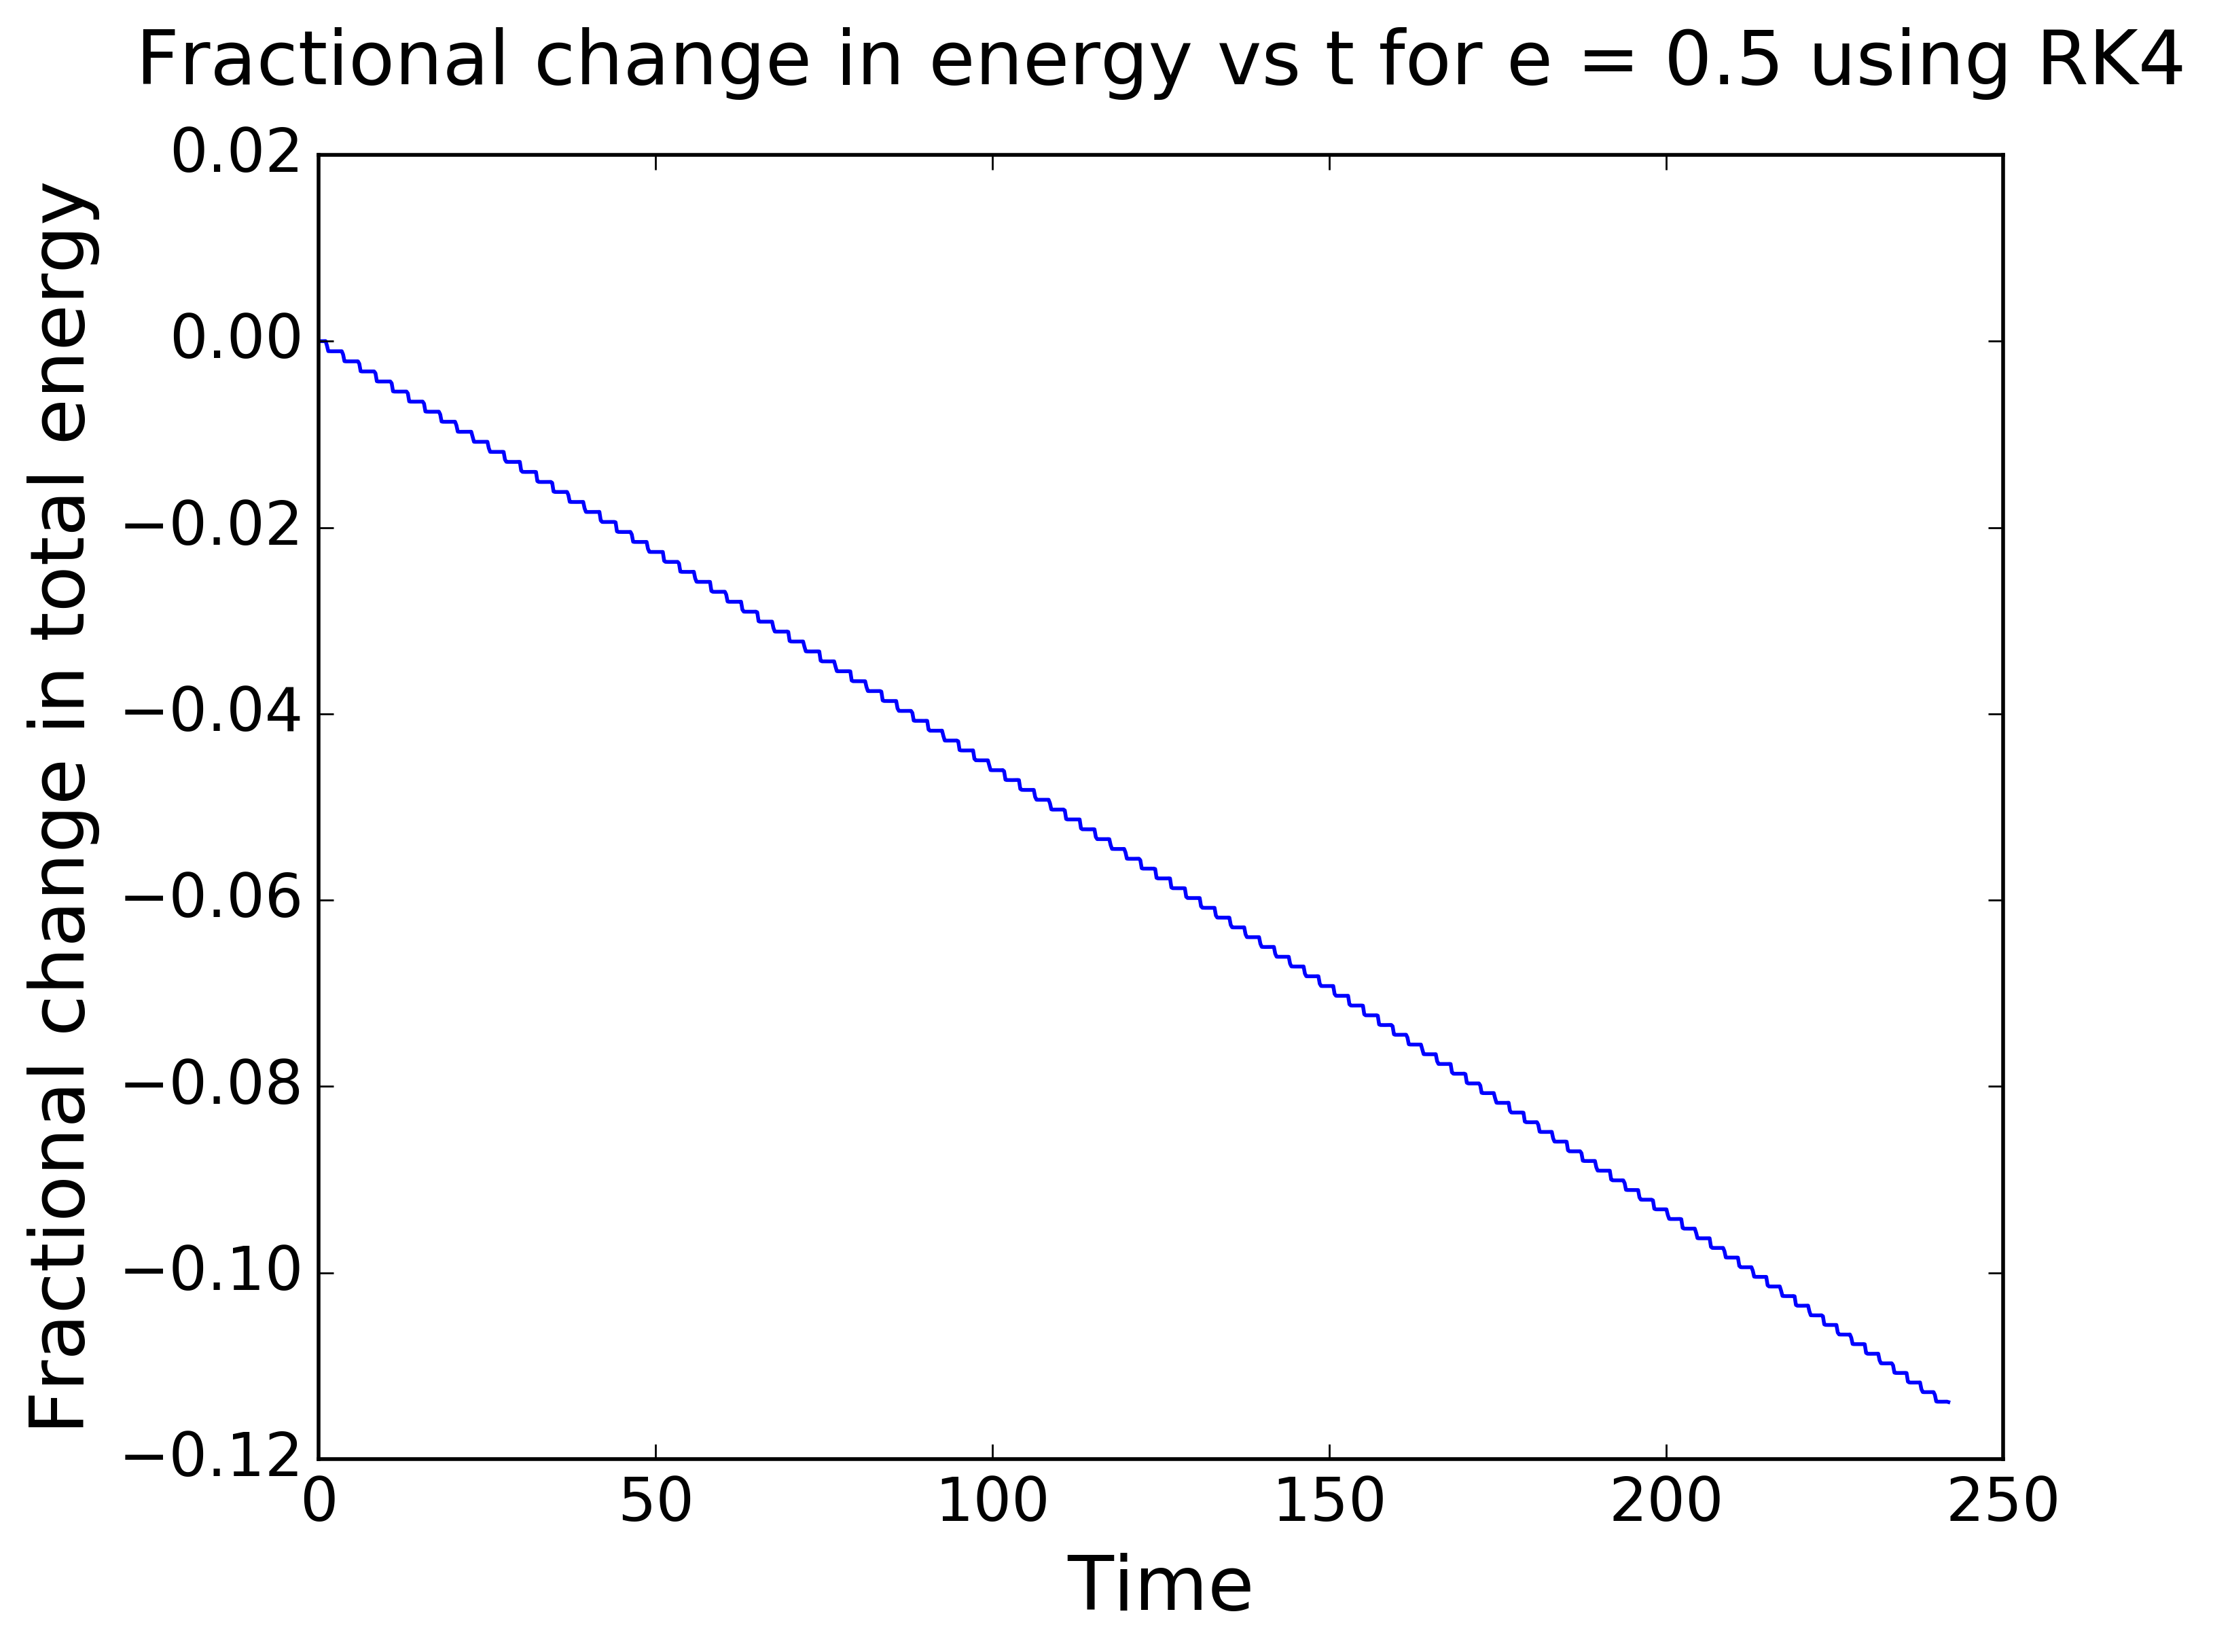
\includegraphics[width=\linewidth]{plots_p1/RK4_e05_energy.png}
	\end{minipage}
\end{figure}



\subsubsection*{2nd order leapfrog vs. 4th order Runge-Kutta for e = 0.9}

\begin{figure}[H]
	\centering
	\begin{minipage}[b]{0.48\linewidth}
		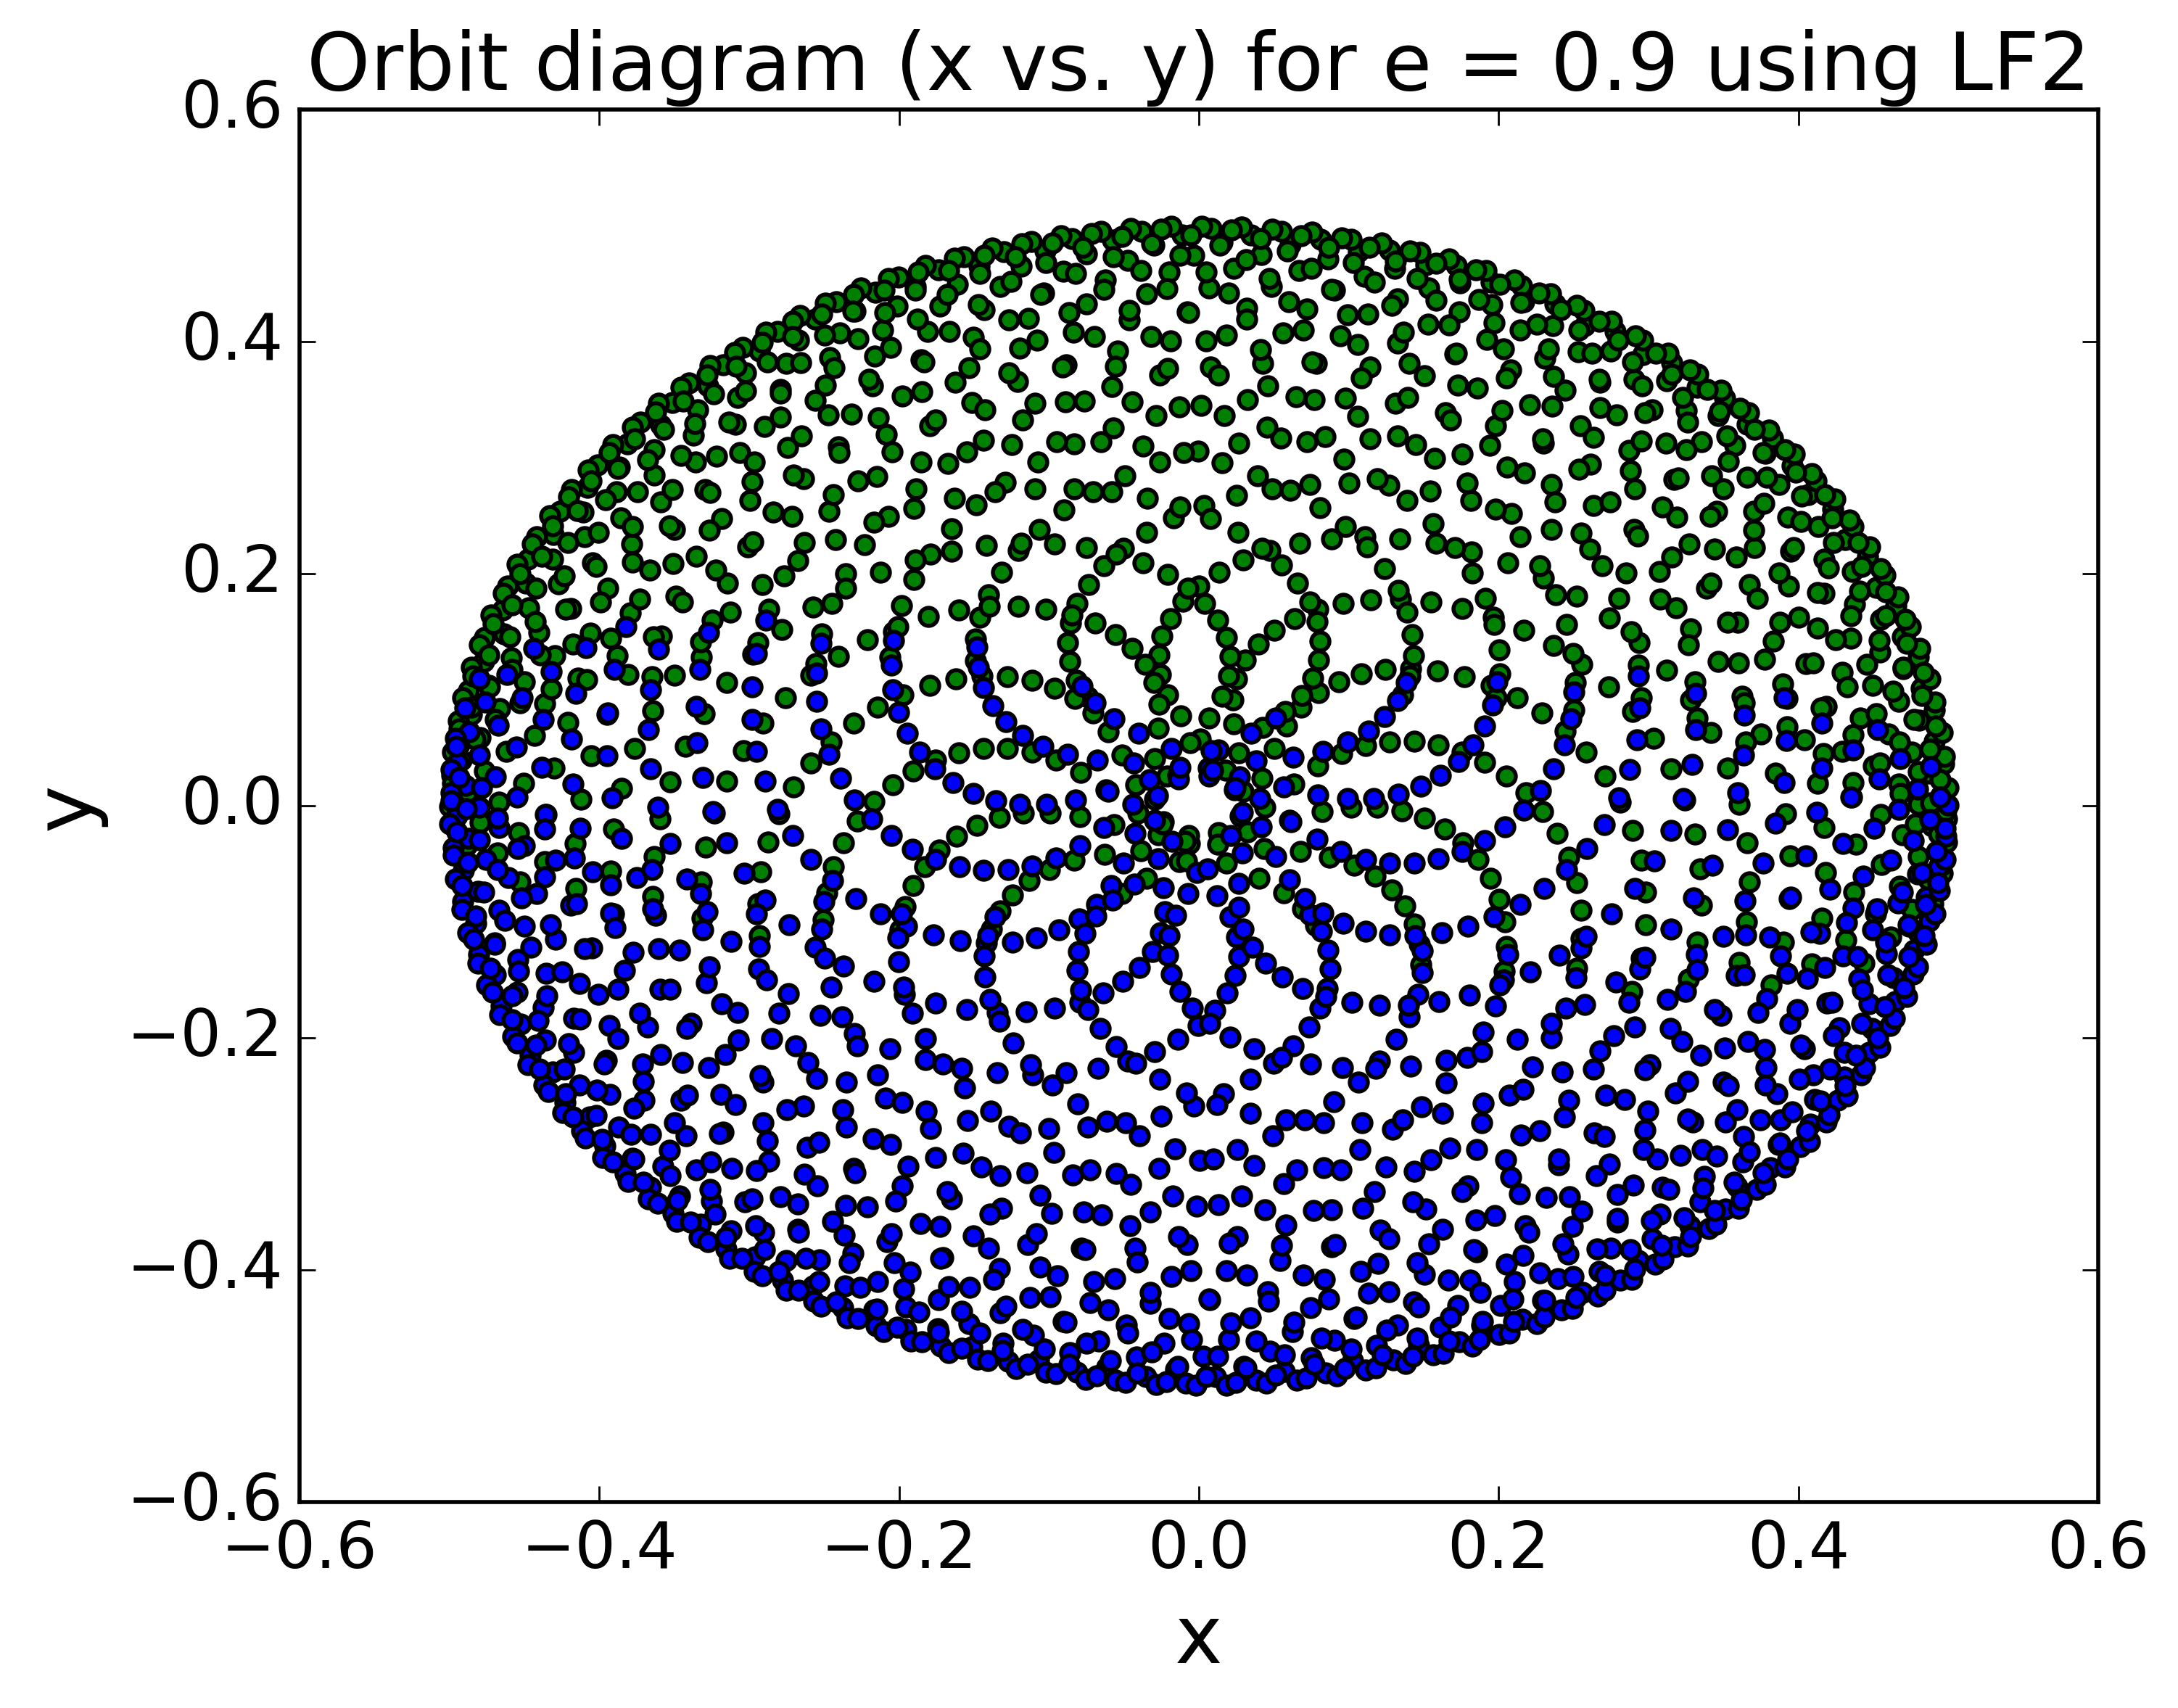
\includegraphics[width=\linewidth]{plots_p1/LF2_e09_xy.png}
		%\caption{\label{fig:lightstd}.}
	\end{minipage}
	%\quad
	\begin{minipage}[b]{0.48\linewidth}
		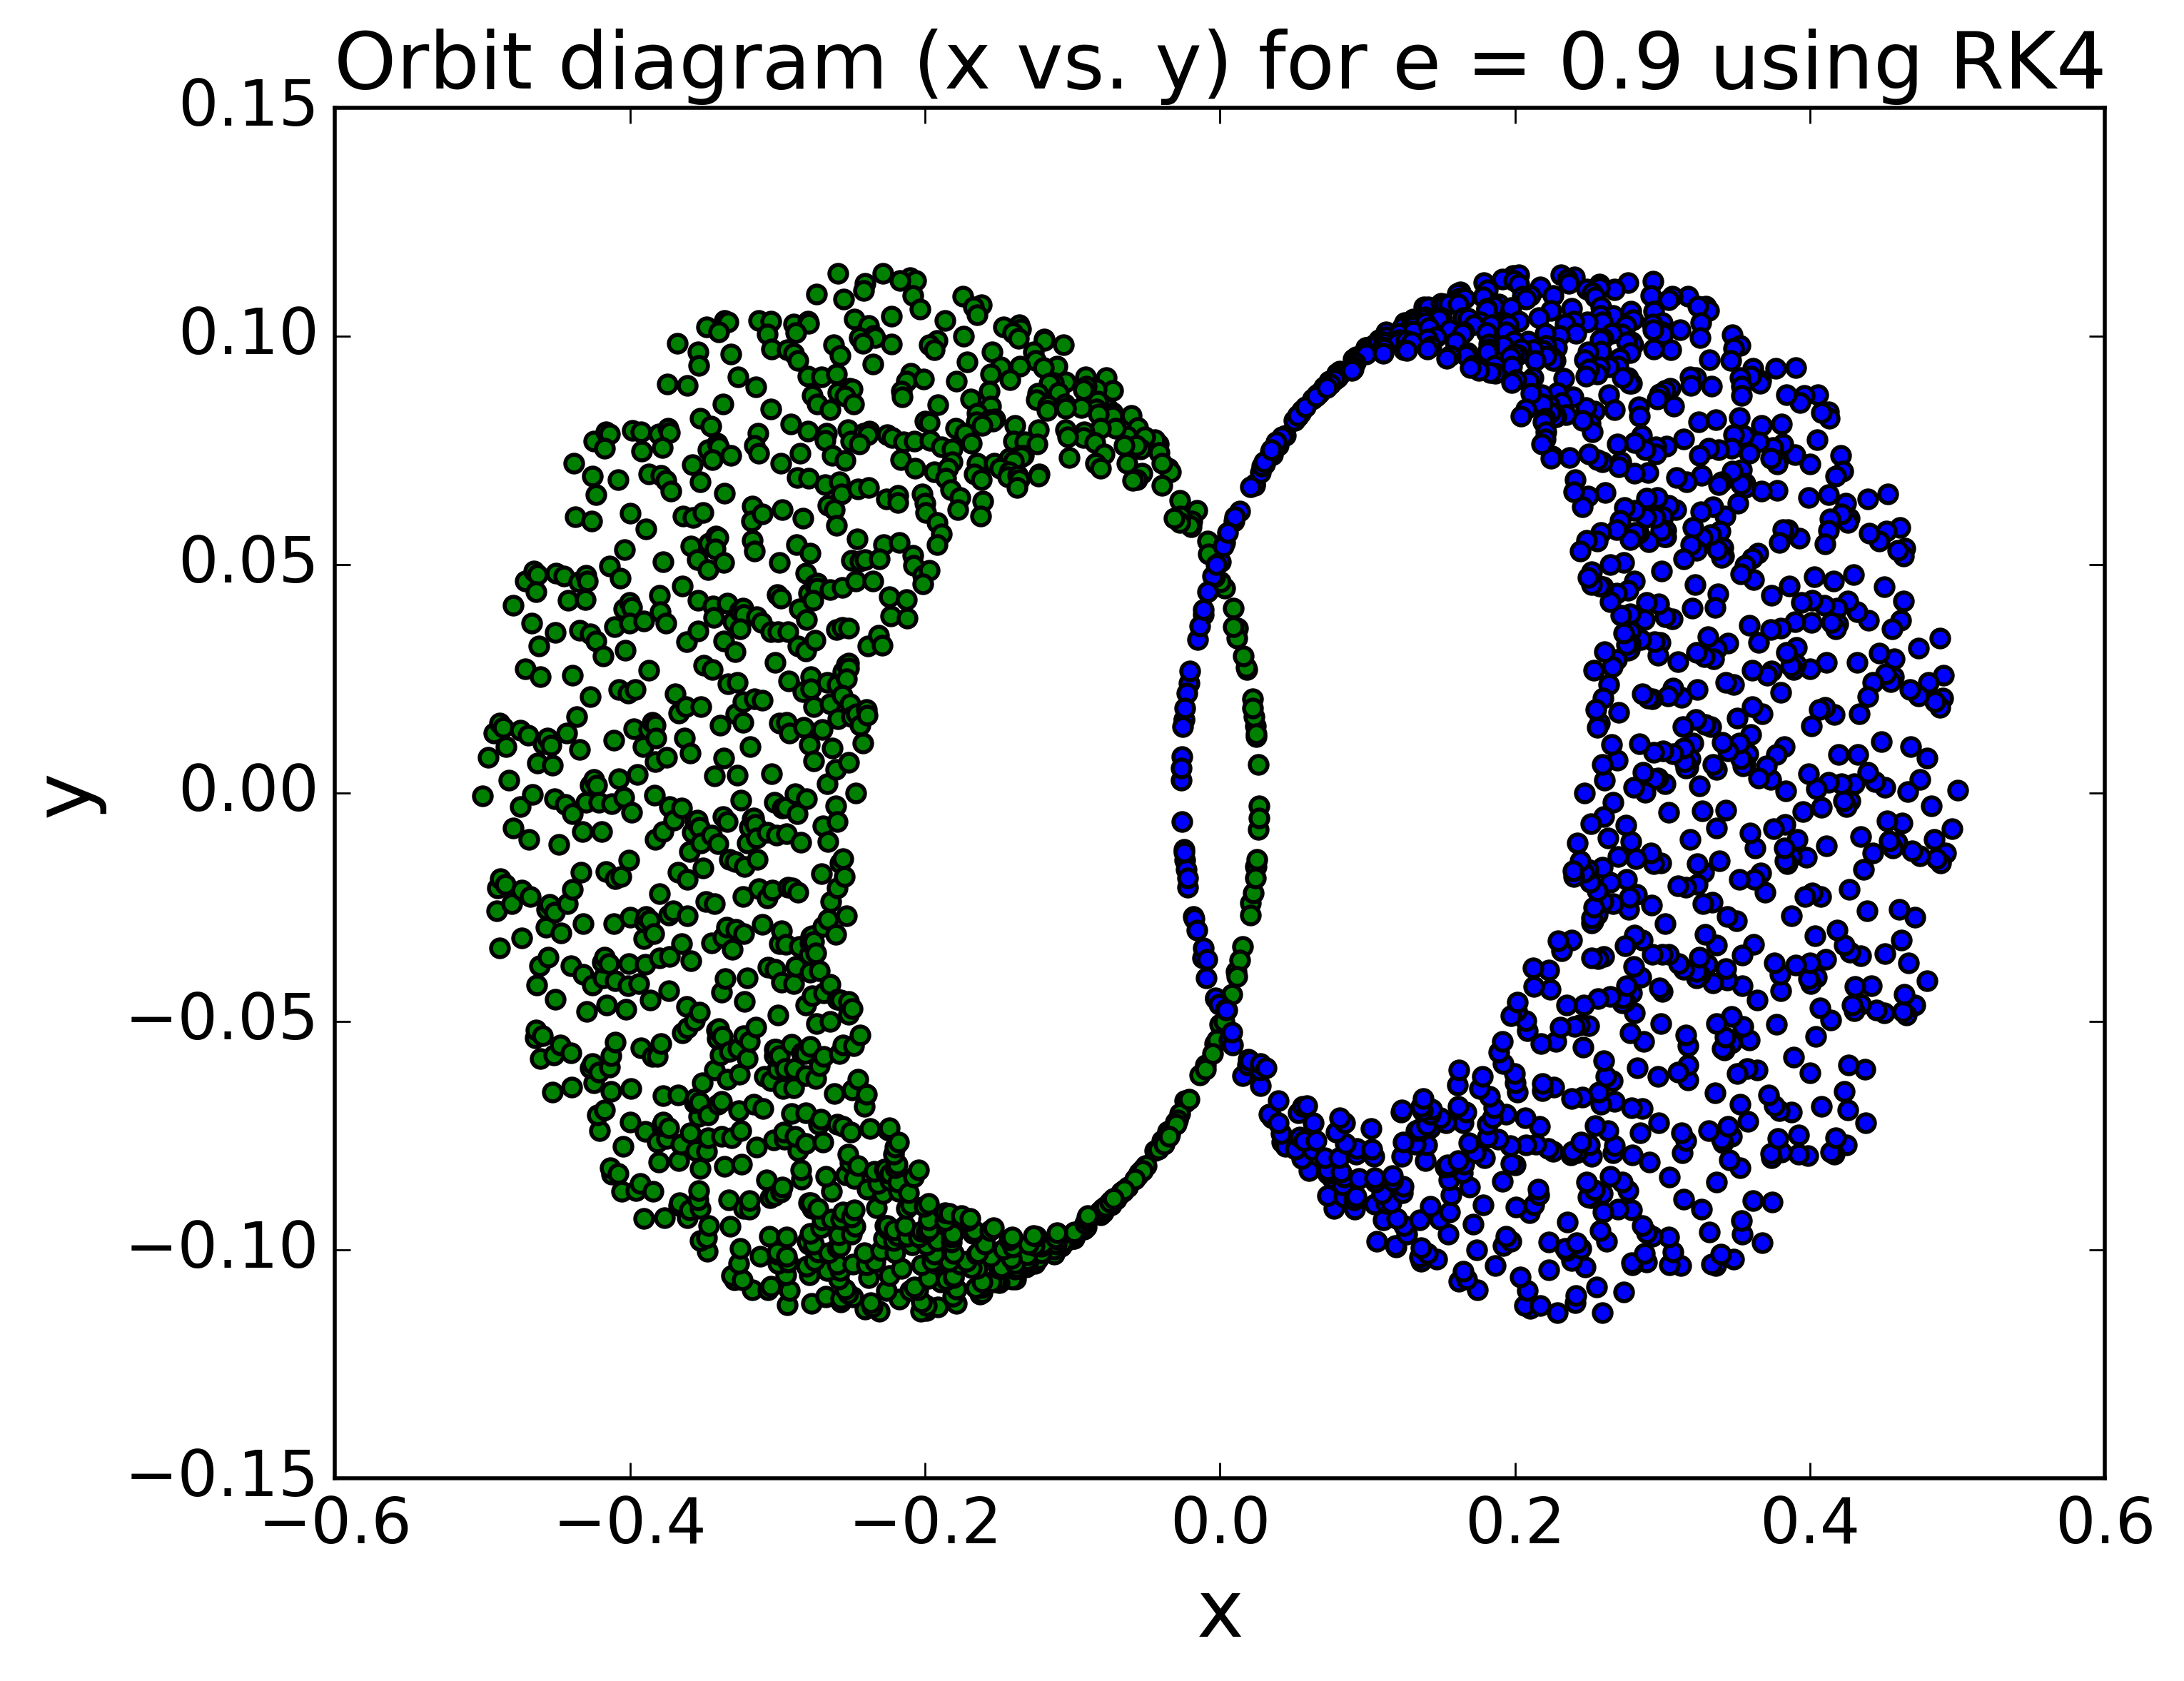
\includegraphics[width=\linewidth]{plots_p1/RK4_e09_xy.png}
	\end{minipage}
\end{figure}

\begin{figure}[H]
	\centering
	\begin{minipage}[b]{0.48\linewidth}
		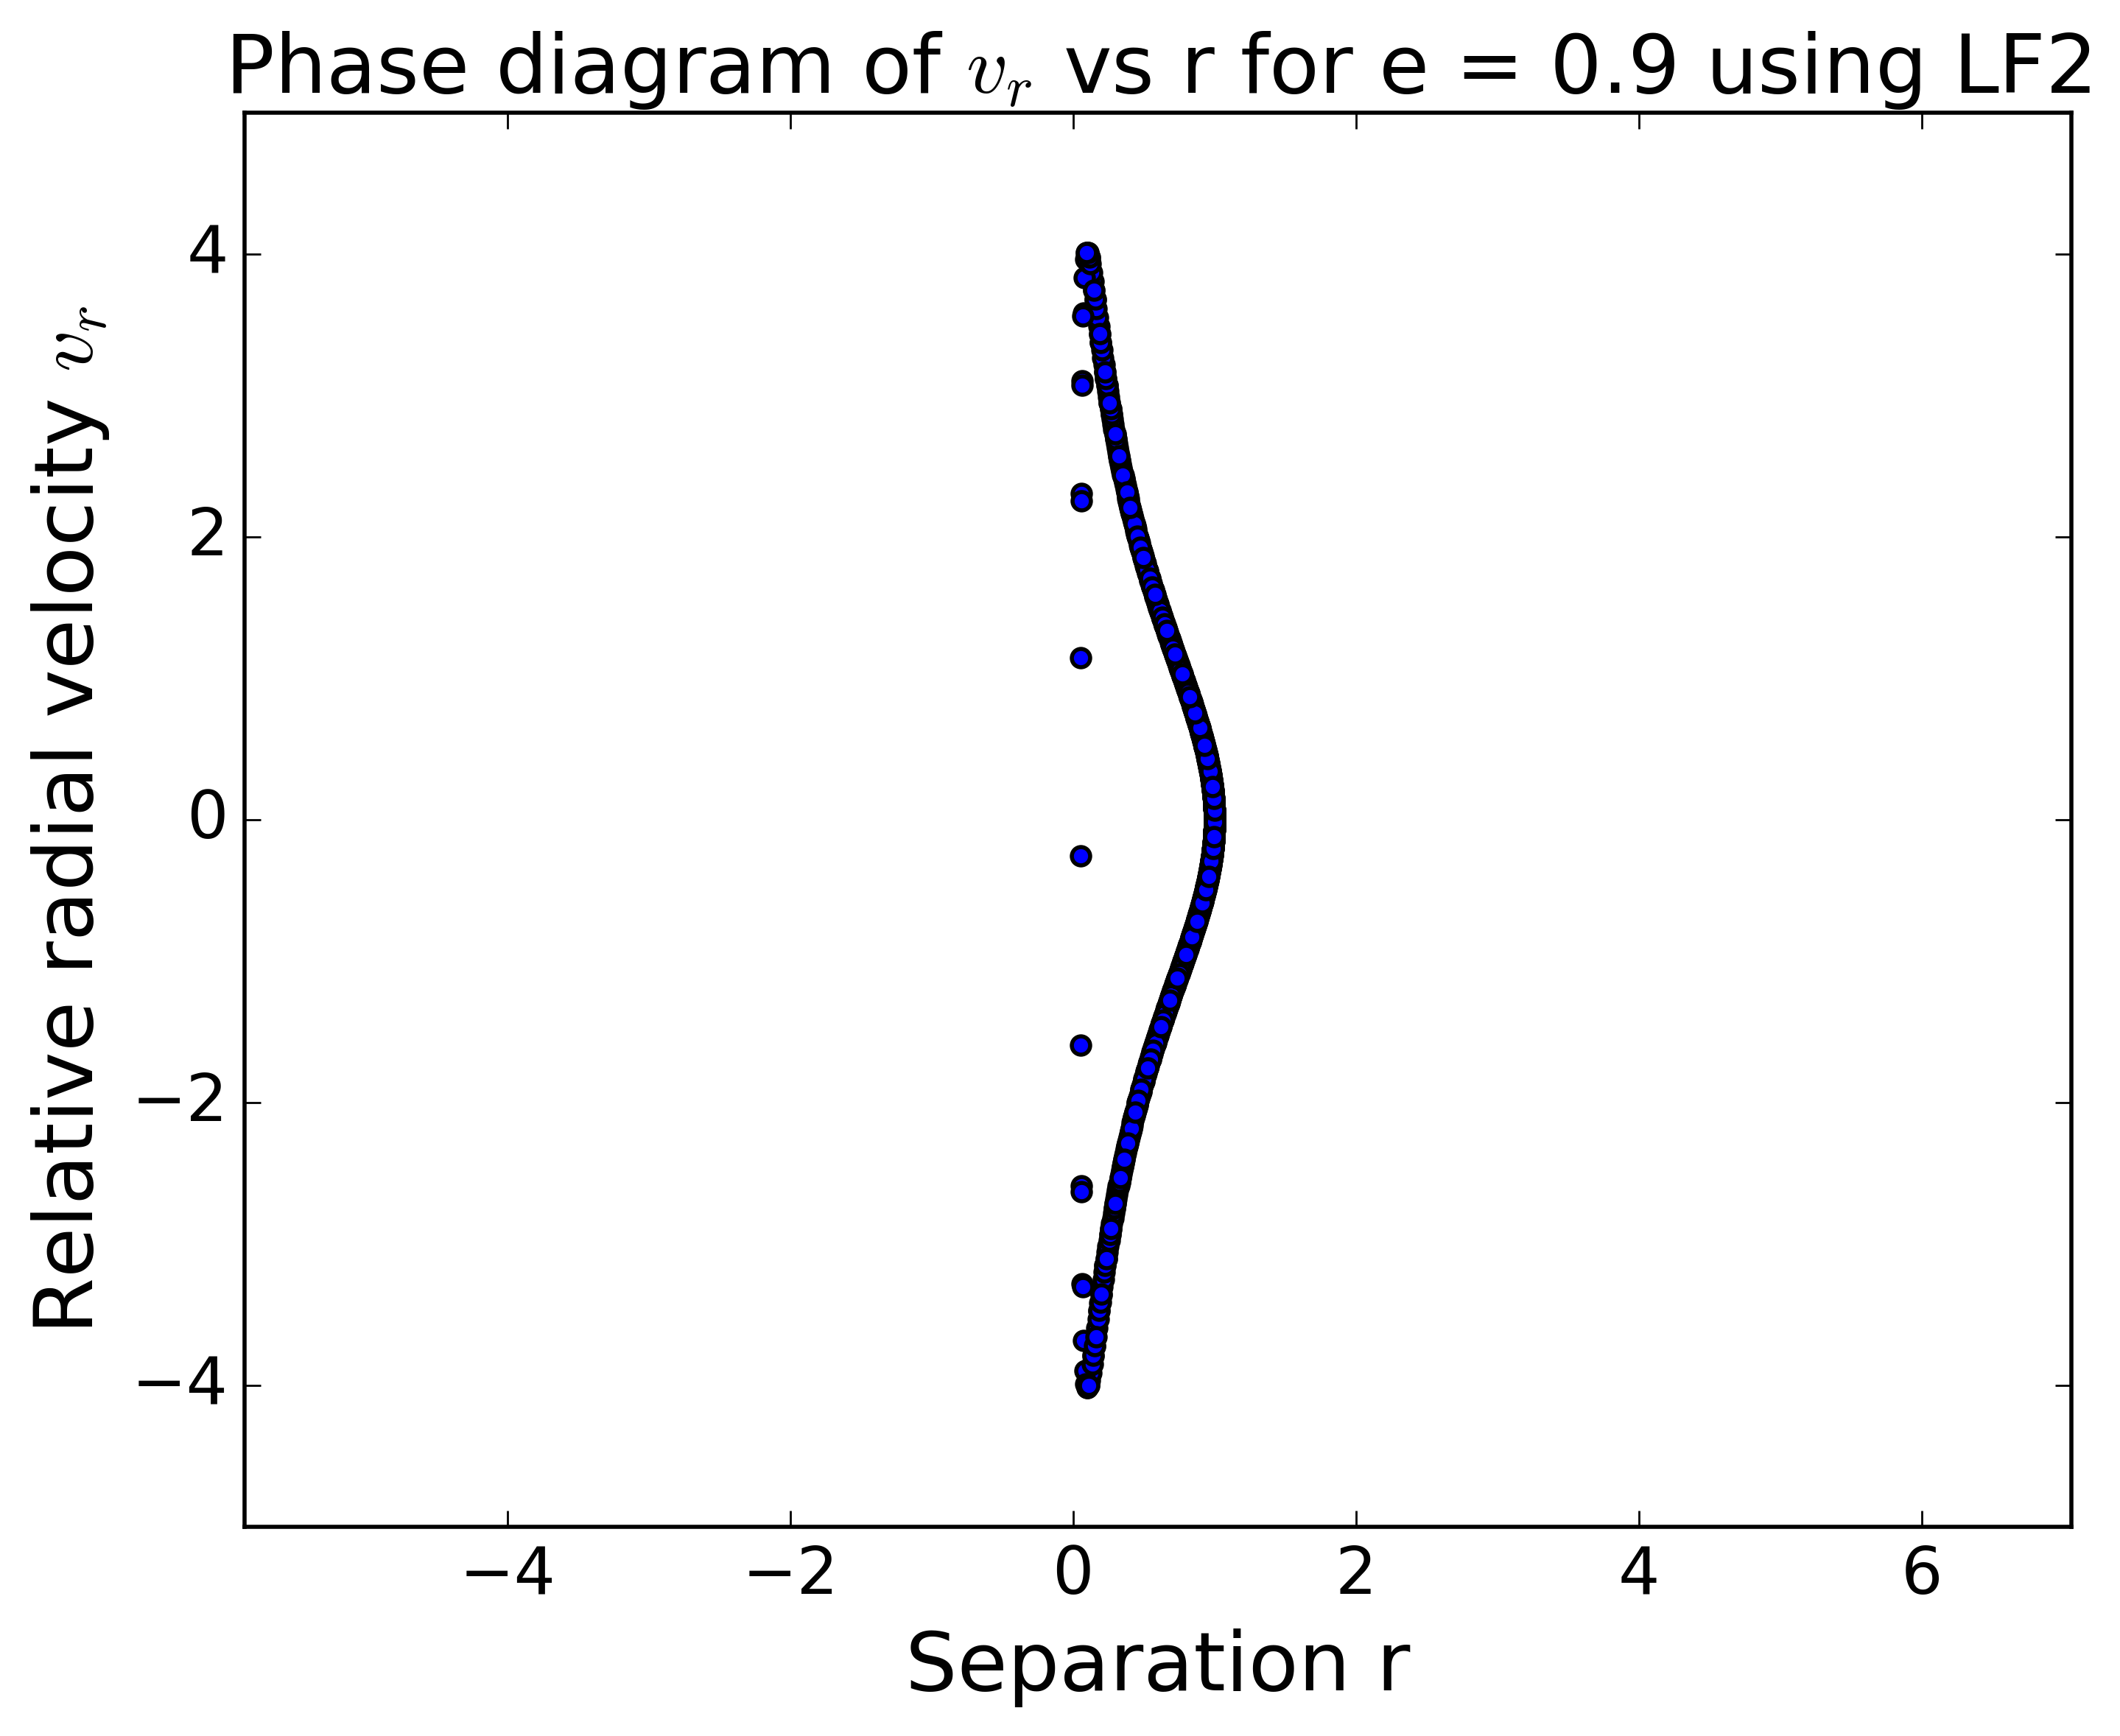
\includegraphics[width=\linewidth]{plots_p1/LF2_e09_rv.png}
		%\caption{\label{fig:lightstd}.}
	\end{minipage}
	%\quad
	\begin{minipage}[b]{0.48\linewidth}
		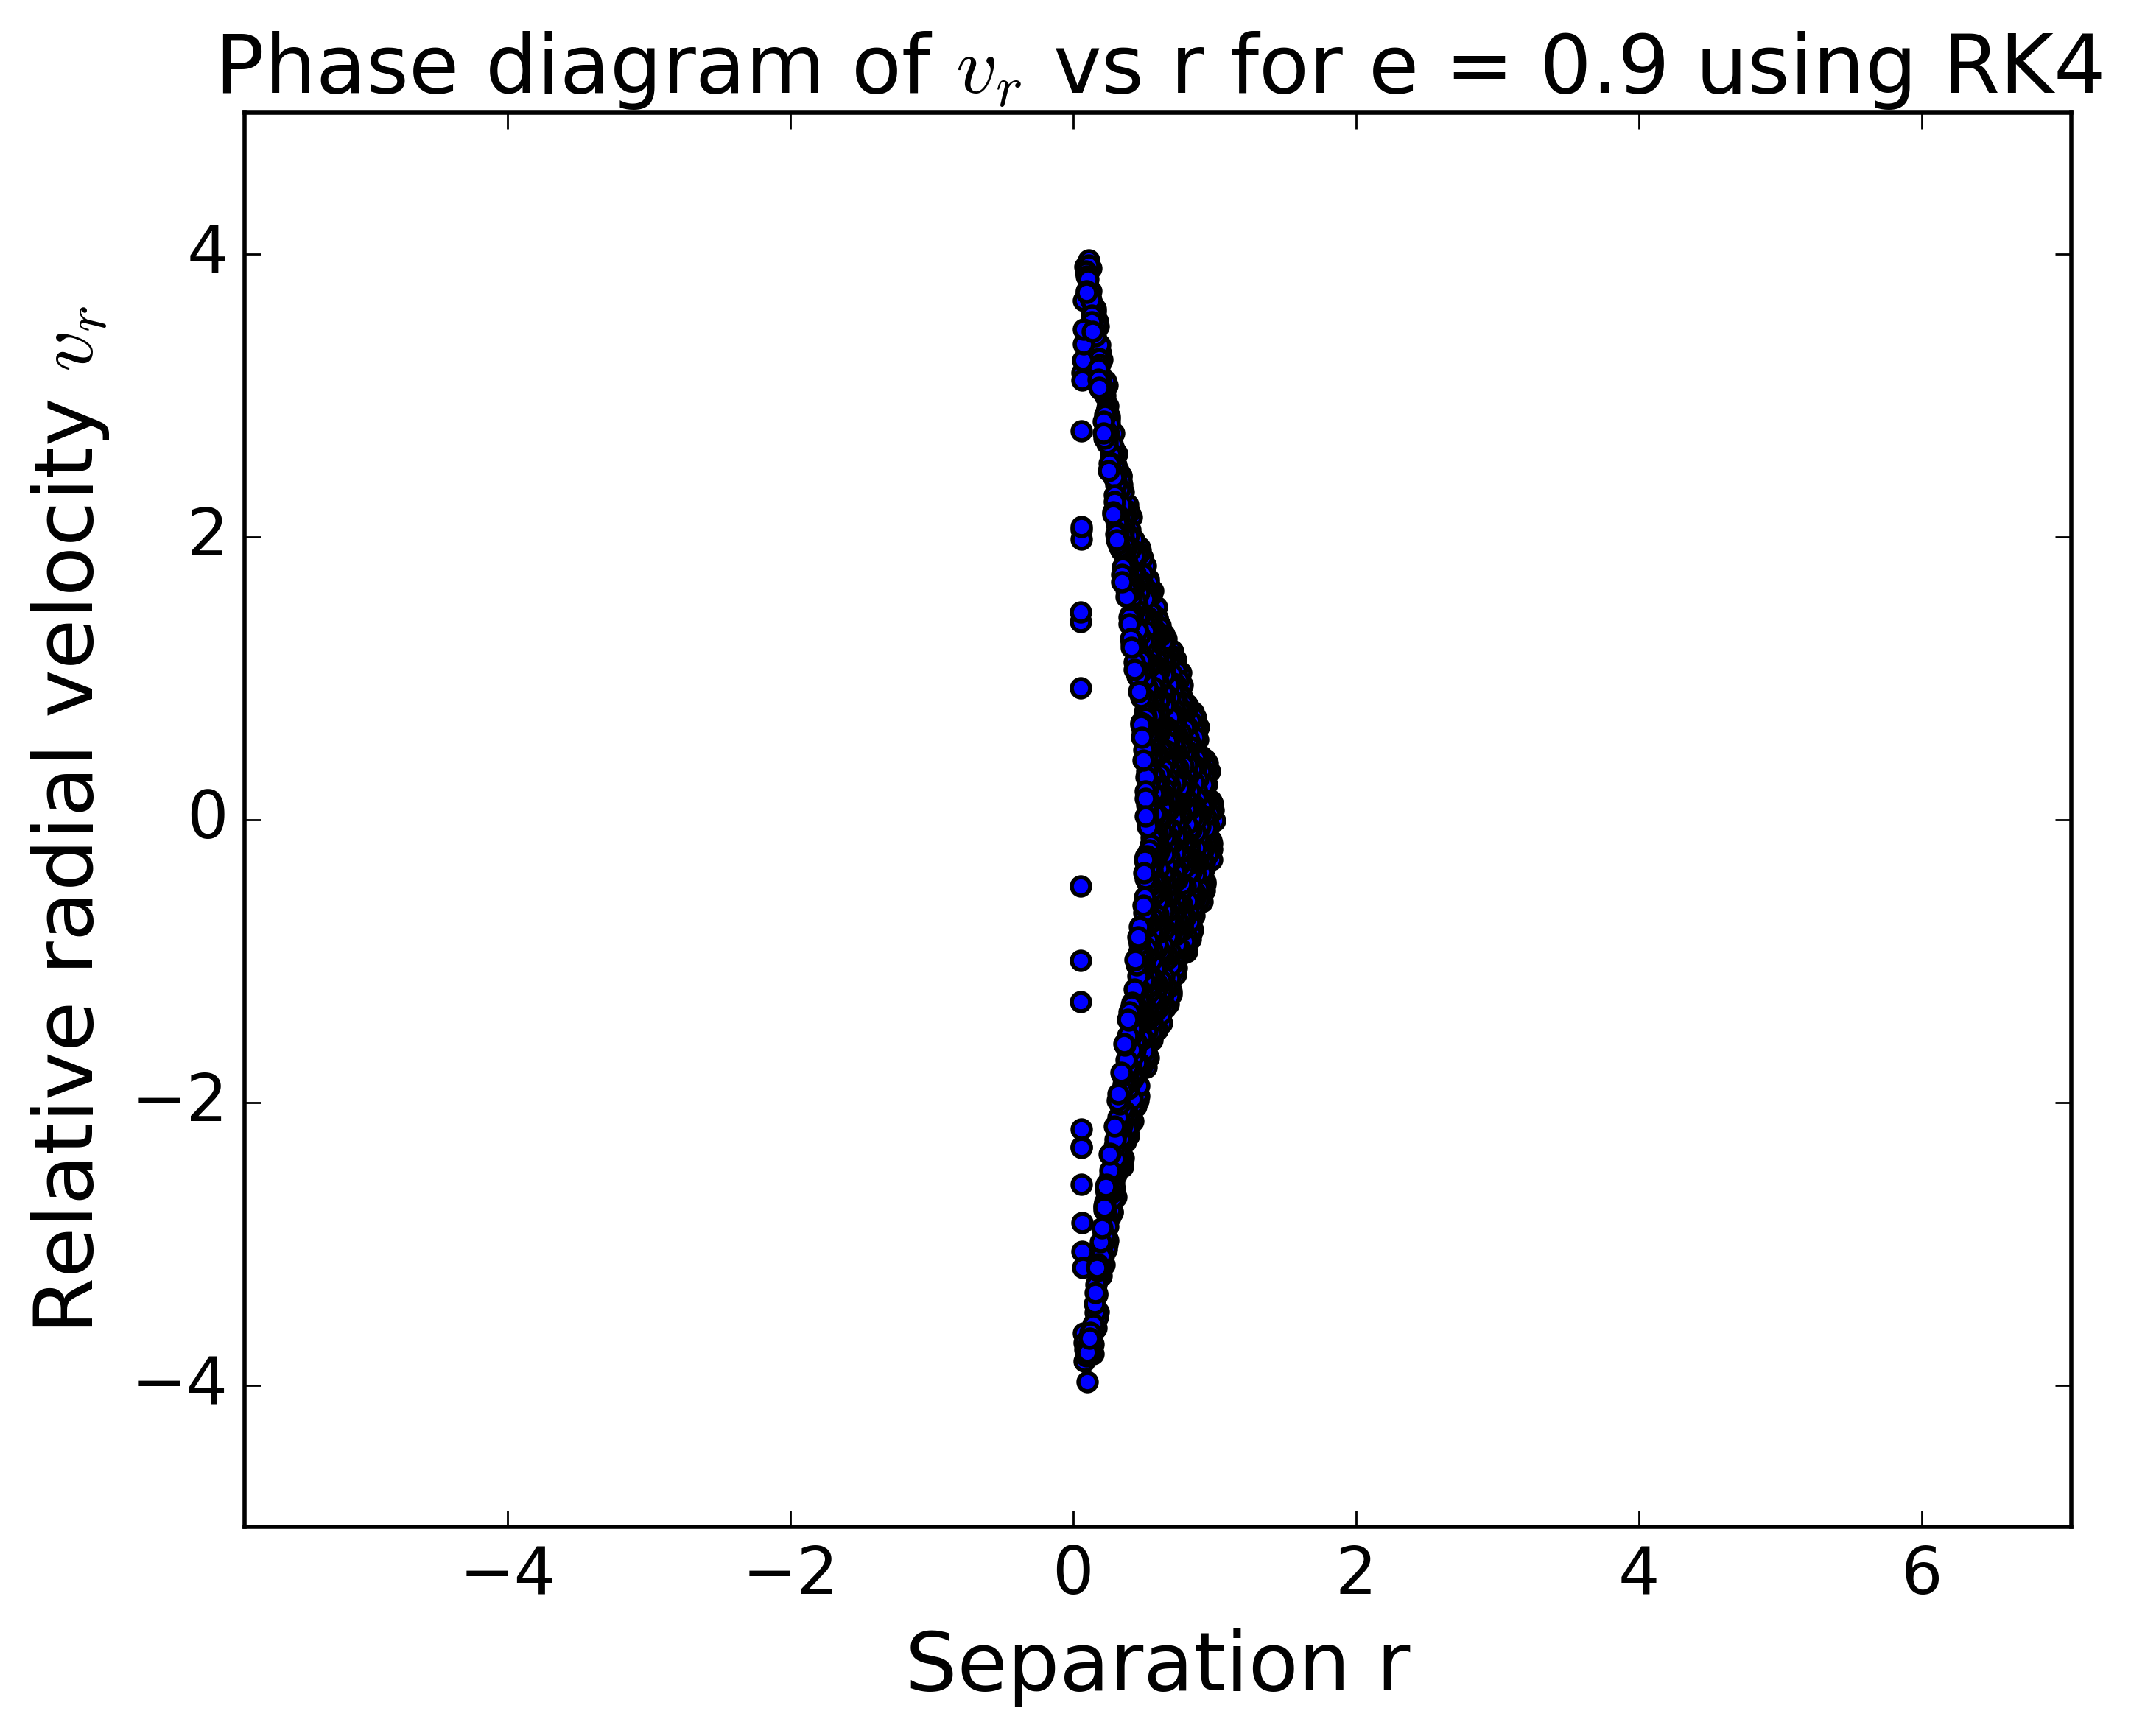
\includegraphics[width=\linewidth]{plots_p1/RK4_e09_rv.png}
	\end{minipage}
\end{figure}

\begin{figure}[H]
	\centering
	\begin{minipage}[b]{0.48\linewidth}
		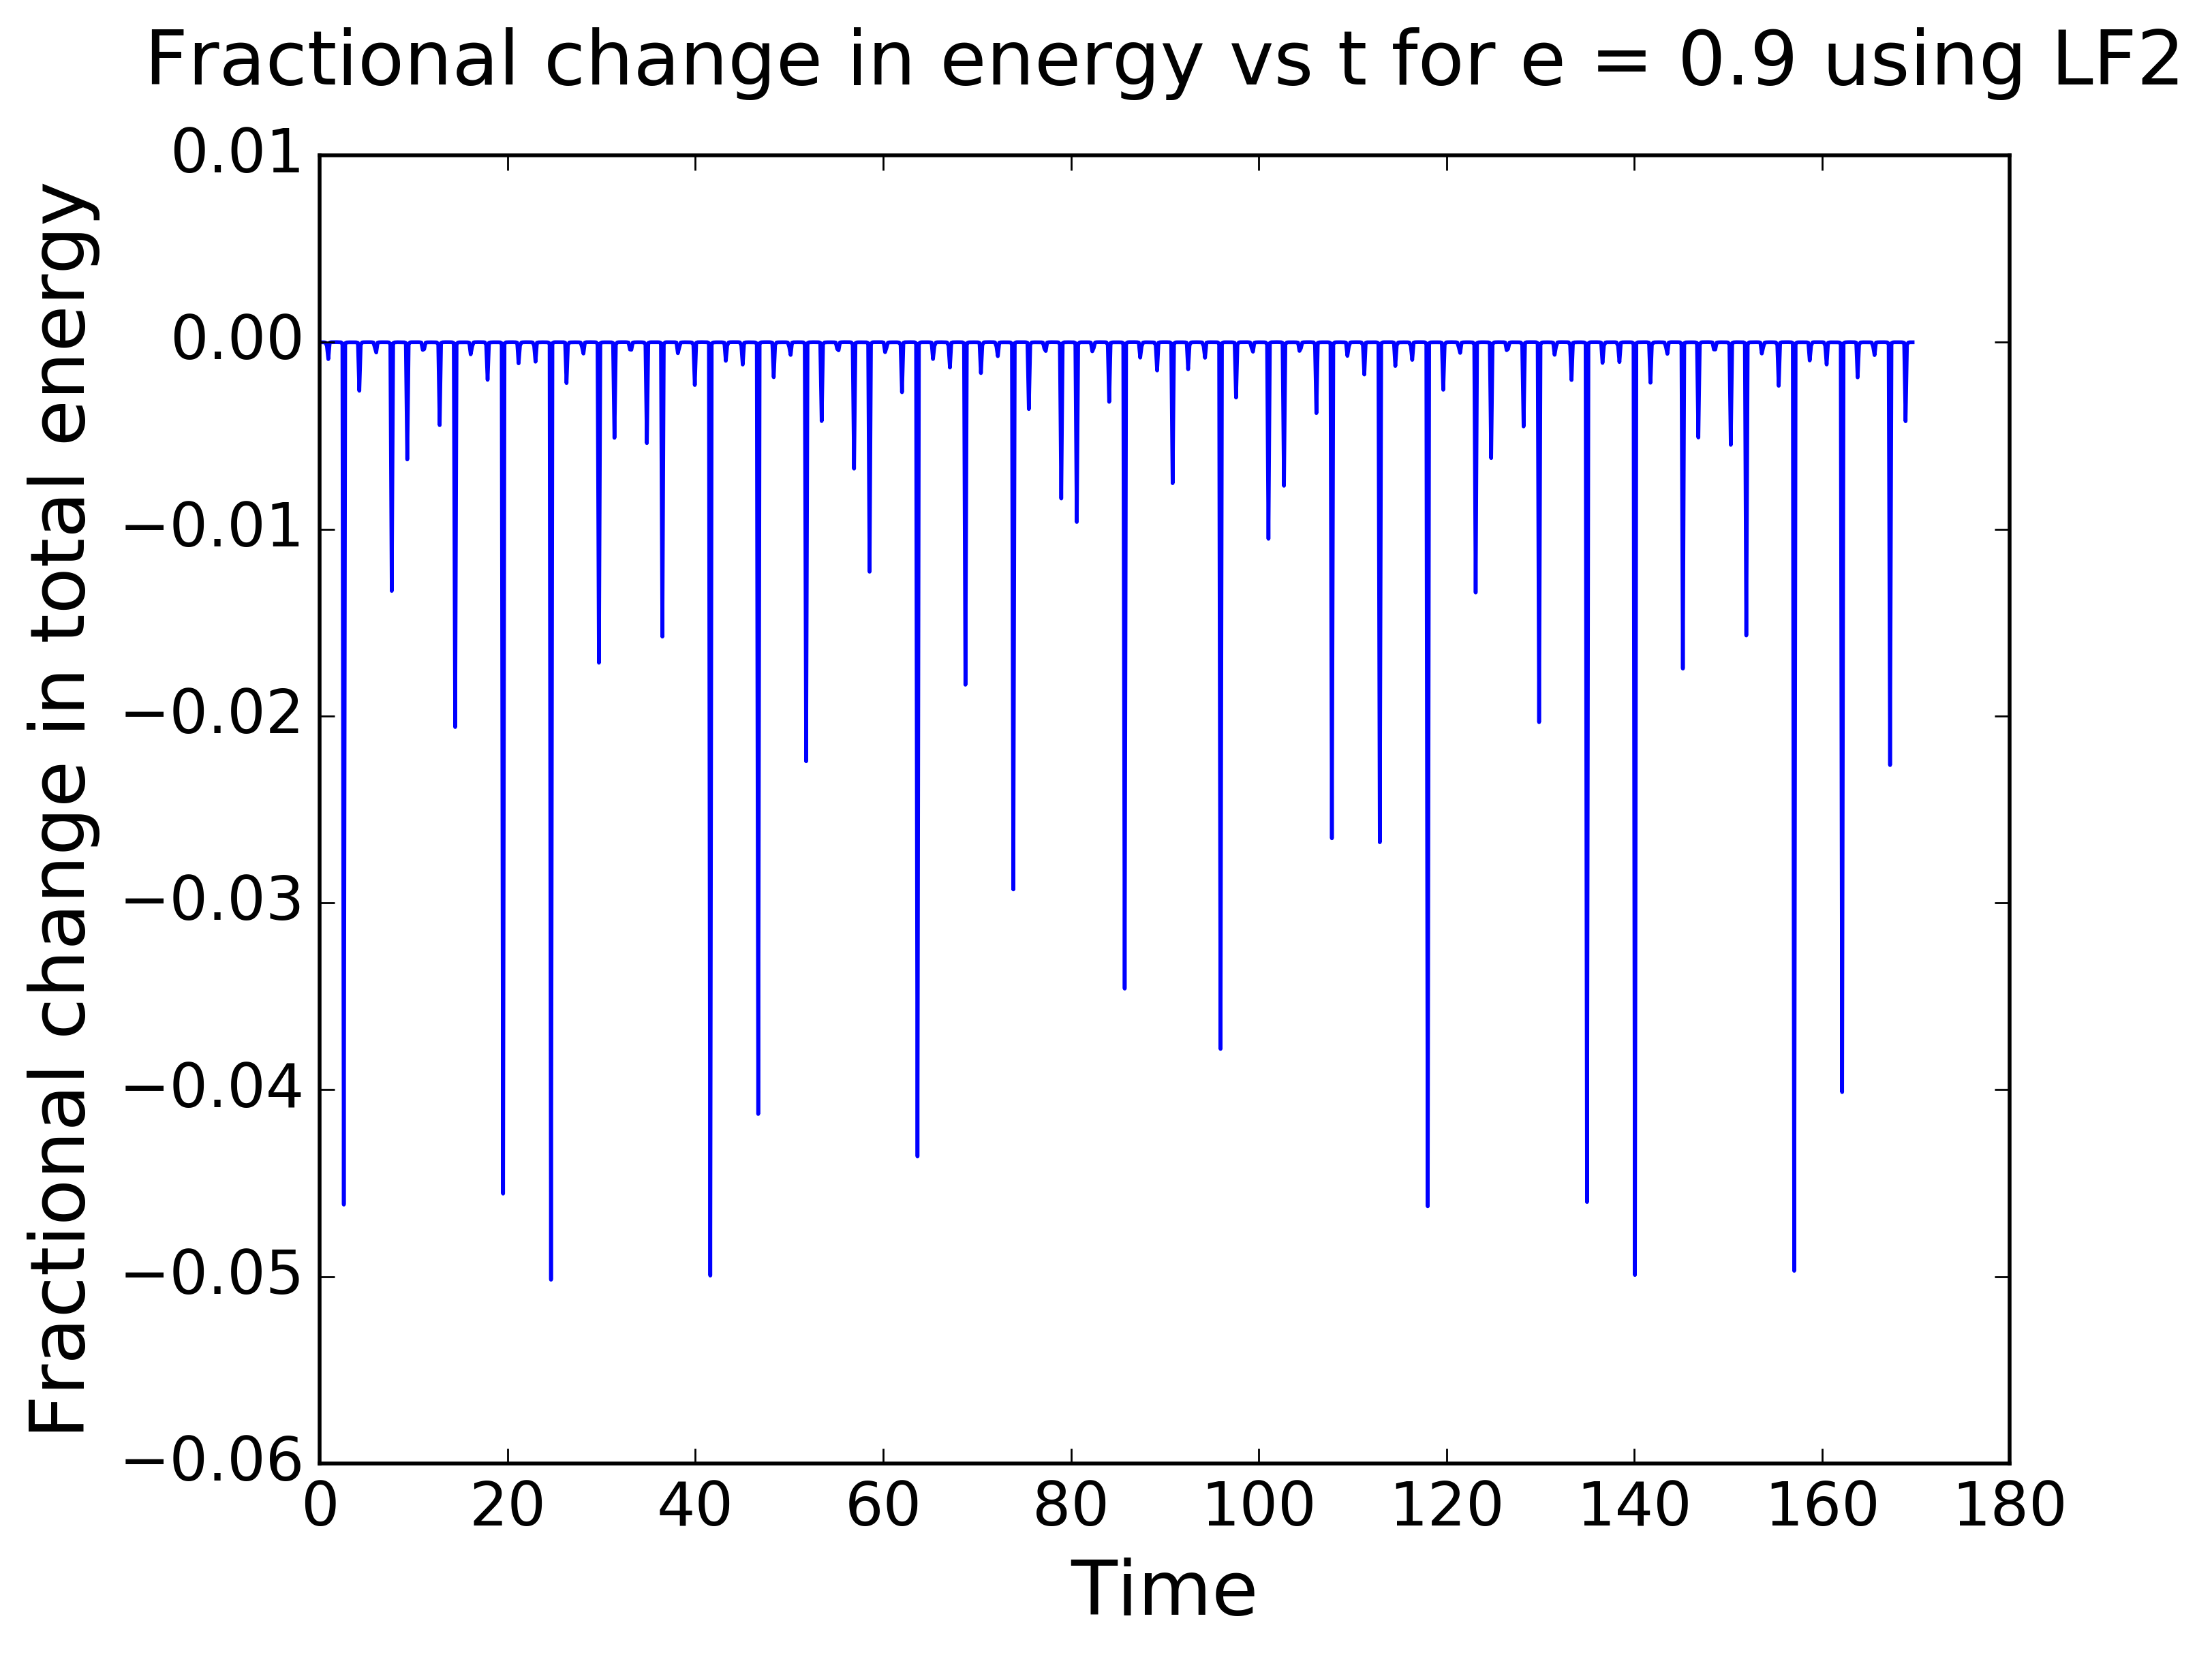
\includegraphics[width=\linewidth]{plots_p1/LF2_e09_energy.png}
		%\caption{\label{fig:lightstd}.}
	\end{minipage}
	%\quad
	\begin{minipage}[b]{0.48\linewidth}
		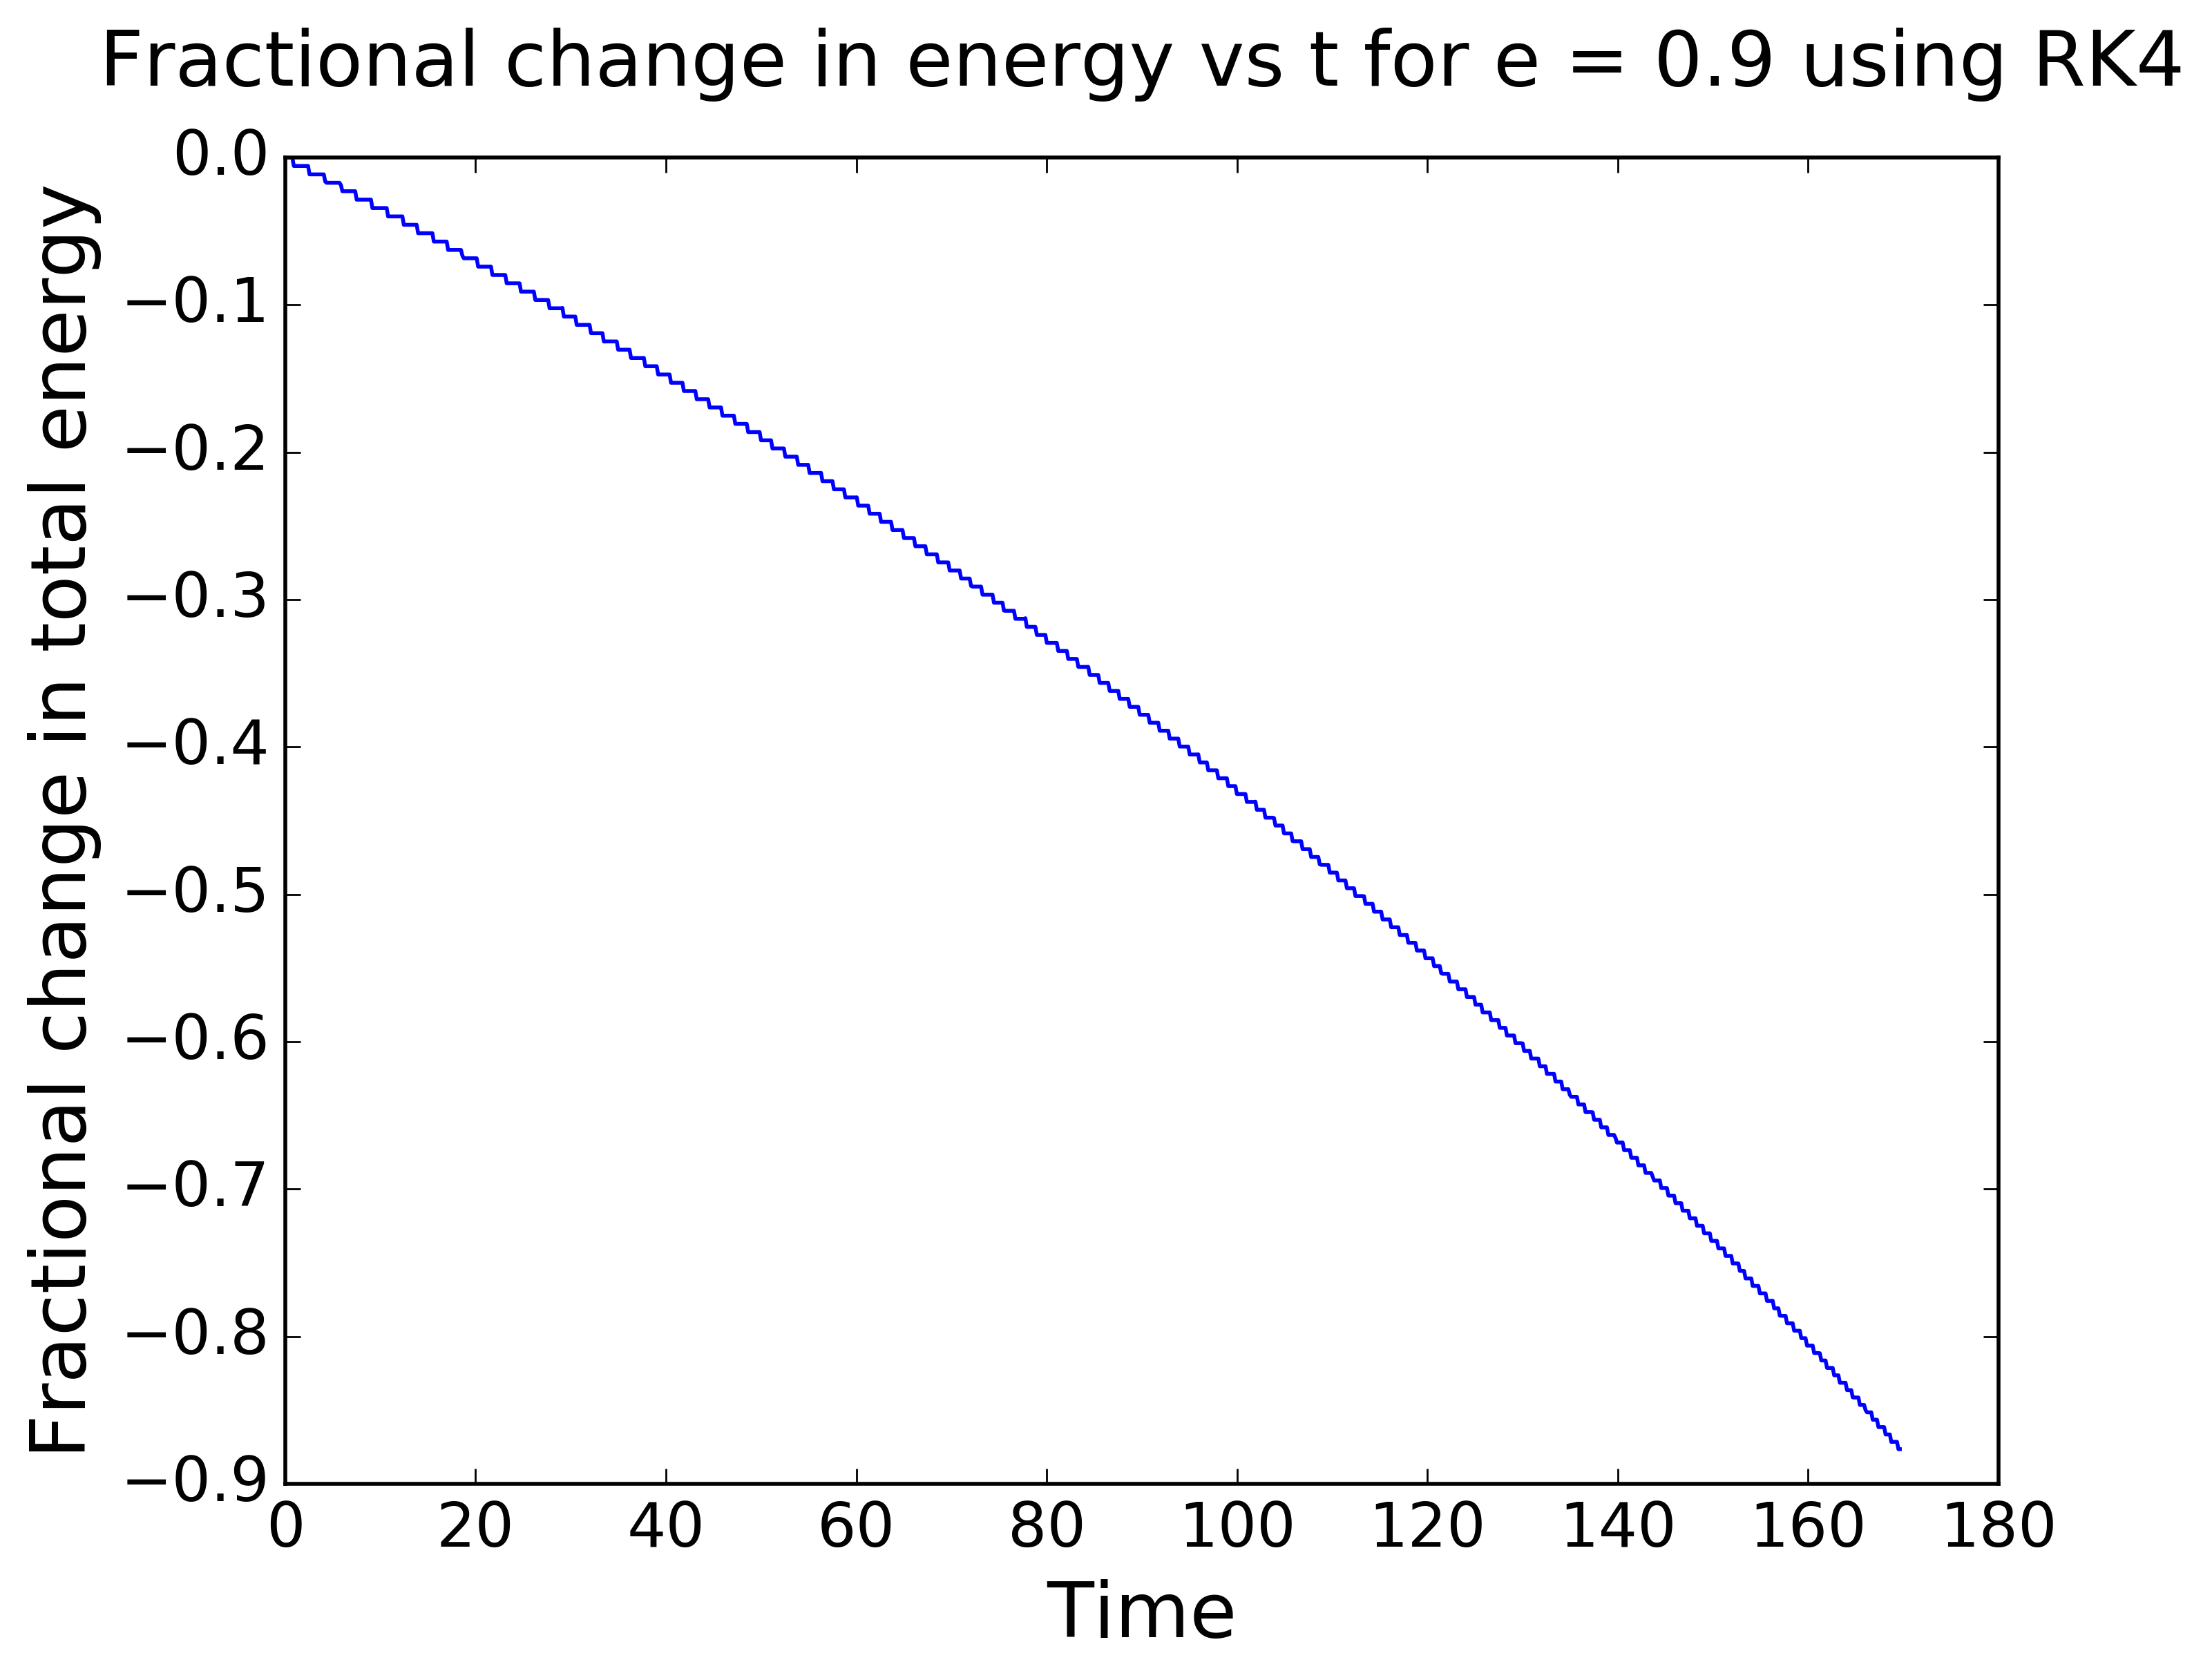
\includegraphics[width=\linewidth]{plots_p1/RK4_e09_energy.png}
	\end{minipage}
\end{figure}



\subsubsection*{Comments}
\begin{itemize}
	\item  Leapfrog is better at conserving energy. For e = 0.9, the energy error in RK4 reaches 90\% after 100 periods. While in LF2, the fractional change in energy oscillates with a maximum error of 5\%.
	
	\item This is also clear from the phase diagram; LF2 repeats almost exactly the same cycle, while RK4 produces larger errors since the separation decreases continually as the system loses energy.
	
	\item LF2 leads to larger phase error than RK4. After 100 periods, the phase error is almost pi/2 for LF2 (at the given time step), while the phase remains almost the same for RK4.
	
	\item Therefore, leapfrog is more practical for N-body simulations with long simulation time, while Runge-Kutta is more accurate for small simulation time. 
	
\end{itemize}

\section*{Problem 2}
We perform a simulation of a cluster with Kroupa IMF.
\subsection*{Mass distribution}
We implement in all of our simulations the Kroupa IMF:
\begin{equation}
\phi(m) \propto 
\begin{cases}
m^{-1.3} \; &(0.08M_\odot < m < 0.5M_\odot) \\
0.5 \, m^{-2.3} \; &(0.5M_\odot<m<100M_\odot)
\end{cases}
\end{equation}
after doing transformation we get
\begin{equation}
m=
	\begin{cases}
	-\cfrac{0.566179}{\sqrt[3]{1.7987\, - x} \left(x^3-5.39611 
	x^2+9.70599 x-5.81939\right)} & (0<x<0.760707)\\
	\cfrac{0.166558}{(1.00024\, -x)^{10/13}} & (0.760707<x<1)
	\end{cases}
\end{equation}

\subsection*{Initial setup}
The cluster is a specially uniformly distributed sphere with a radius of 1. The inital 
velocities are from a  Gaussian distribution with a dispersion correspondent to a virial ratio 
of $ \alpha \sim 0.4 $. A virial ratio $ \alpha < 0.5 $ implies the system is bounded. The 
velocity dispersion crossing time is $ t \approx 0.08 $, so we use a step size of 0.001, i.e. 
80 steps per course time.

\subsection{Video}
The video of this specific setup is \textit{simulations/cluster03.mp4}.

%../pp-nbody/a.out cluster03.txt cluster03 1000 0.01 0.001 200 1


%\subsection*{Morphology}
%We use disk galaxies in our simulation. Each disk galaxy has two components: a 
%thin disk and a thick disk. Each component has a density profile $ \rho(r, h) = 
%\rho_0 \, e^{-r/r_{\rm H}} \, e^{-h/h_{\rm H}} $. $ r $ and $ h $ are given by the 
%solution to the equation
%\begin{equation}\label{key}
%	x = 1 - (1 + \frac{r}{r_{\rm H}}) \, e^{-\frac{r}{r_{\rm H}}}
%\end{equation}
%where $ x $ is a uniform random number between 0 and 1.
%
%\subsection*{Disk Rotation}
%We use a uniform angular velocity $ \omega $.

%\subsection*{Setups}
%\begin{table}[h]
%	\centering
%	\begin{tabular}{ccccc}
%%		\hline{}
%		& $M/M_\odot$ & $r_{\rm H}$/kpc & $h_{\rm H} $/kpc & $\omega/?$ \\
%		\hline
%		thin disk & $5 \times 10^{10}$ & 3.5 & 0.3 & 1? \\
%		thick disk & $ 0.75 \times 10^{10} $ & 3.5 & 1.0 & 1? \\
%%		\hline
%	\end{tabular}
%	\caption{Parameters and errors from Lorentzian and Gaussian fits.}
%	\label{fit params}
%\end{table}
%
%\subsection{Units}
%[L] = kpc, [M] = $ 10^9 M_\odot $, [T] = 14.91 Myr.


\end{document}